% %%%%%%%%%%%%%%%%%%%%%%%%%%%%%%%%%%% %
% Template criado por @Guvidaletti    %
% Utilizando o template da AGES v2.1  %
% como base                           %
% %%%%%%%%%%%%%%%%%%%%%%%%%%%%%%%%%%% %

% Configuração do Documento
\documentclass[
  a4paper,
  12pt,
  oneside,
  chapter=TITLE,
  english,
  brazil]
  {abntex2}

\usepackage[brazil]{babel}

\usepackage[
  tmargin=3cm,
  lmargin=3cm,
  bmargin=2cm,
  rmargin=2cm,
]{geometry}


% Para utilizar imagens dentro do LaTeX:
\usepackage{graphicx}

% \usepackage{lmodern}			% Usa a fonte Latin Modern
\usepackage{helvet}             % Usa a fonte Helvetica
\usepackage[T1]{fontenc}		% Selecao de codigos de fonte.

% Para utilizar fontes diferentes:
% Define Sans Serif para todo documento
\renewcommand{\familydefault}{\sfdefault}

% Deve haver recuo no primeiro paragrafo
\usepackage{indentfirst}

% Capitulos, secoes e subsecoes devem ter tamanho normal
\renewcommand{\ABNTEXchapterfontsize}{\normalsize}
\renewcommand{\ABNTEXsectionfontsize}{\normalsize}
\renewcommand{\ABNTEXsubsectionfontsize}{\normalsize}
\renewcommand{\ABNTEXsubsubsectionfontsize}{\normalsize}

% Capitulos e secoes devem estar negritados
% https://groups.google.com/g/latex-br/c/ULm17Zfng3w/m/ZbCHIHLi7GAJ
\renewcommand{\ABNTEXchapterfont}{\normalfont\sffamily\bfseries}
\renewcommand{\ABNTEXsectionfont}{\normalfont\sffamily\bfseries}
% Subsecoes nao devem estar negritados
\renewcommand{\ABNTEXsubsectionfontsize}{\normalfont\sffamily}

% Espacamento vertical entre titulo do capitulo e conteudo deve ser de 24pts
\setlength\afterchapskip{24pt}

% Define colores para links
\hypersetup{
    colorlinks=true,
    linkcolor=black,
    citecolor=black,
    urlcolor=black,
}

% Páginas sem cabeçalho
\pagestyle{simple}

% Subseção não no sumário: (para ir, trocar para 2)
\addtocontents{toc}{\protect\setcounter{tocdepth}{1}}

% Captions com negrito
% \usepackage[font=bf]{caption}
% Caption pequena, com o "Figura" em negrito
\usepackage[font=small,labelfont=bf]{caption}

% Posicionamento de Figuras - Importantíssimo
\usepackage{float}

% Espaçamento de 1,5
\renewcommand{\baselinestretch}{1.5}


% Para a lista de abreviaturas:
\usepackage[printonlyused,withpage]{acronym}

% Se o style=abnt não funcionar, utilize o style=numeric
\usepackage[style=abnt]{biblatex}
\usepackage{csquotes}
\addbibresource{bibliografia/bibliografia.bib}

% Ajuste de ordenação dos arquivos:
\begin{document}
  \author{Gustavo}

\def\autor{\uppercase{Pedro Castiglia Filipetto}}
\def\inicio{2025}
\def\fim{2025}
\def\ages{I}
\def\local{Porto Alegre, Rio Grande do Sul}
\def\ano{2025}

\begin{capa}
  \centering
    \uppercase{
      PONTIFÍCIA UNIVERSIDADE CATÓLICA DO RIO GRANDE DO SUL\\
      ESCOLA POLITÉCNICA\\
      CURSO DE BACHARELADO EM ENGENHARIA DE SOFTWARE\\
      AGES $-$ AGÊNCIA EXPERIMENTAL DE ENGENHARIA DE SOFTWARE\\
      }

    \vfill
    \autor\\
    \vfill
    \textbf{
      \uppercase{
        Memorial de atuação na Agência Experimental de Engenharia de Software 
        {-} Semestre 2025/2
        \\AGES \ages\
      }
    }
    
    \vfill

    \vfill
    \local\\
    \ano\
  \end{capa}
  % Opcional:
  %\def\textoDedicatoria{
  Dedicatória: Texto no qual o autor
  do trabalho oferece homenagem ou
  dedica o seu trabalho a alguém.
}

\begin{dedicatoria}
  \textbf{Dedicatória}
  \vfill
  % Dedicatória:
  \hfill{}
  \parbox{6cm}{
    \begin{flushright}
      \textoDedicatoria\
    \end{flushright}
      }
\end{dedicatoria}
  % Opcional:
  %\begin{agradecimentos}[\protect\bfseries Agradecimentos]
  % Agradecimentos - Inicio
  Os agradecimentos devem ser dirigidos àqueles que contribuíram de maneira
relevante à elaboração do trabalho, restringindo-se ao mínimo necessário, como
instituições (CNPq, CAPES, PUCRS, empresas ou organizações que fizeram parte
da pesquisa), ou pessoas (profissionais, pesquisadores, orientadores, etc.).

Os agradecimentos devem ser colocados de forma hierárquica de importância
e para trabalhos financiados com recursos de instituições (CAPES, CNPq, FINEP,
FAPERGS, etc.) os agradecimentos são obrigatórios a essas instituições.
  % Agradecimentos - Fim
\vfill
\end{agradecimentos}
  % Opcional:
  %\def\textoEpigrafe{
  Epígrafe: É um item onde o autor 
  apresenta a citação de um texto 
  que seja relacionado com o tema
  do trabalho, seguido da indicação 
  de autoria do mesmo.\ (texto iniciando 
  do meio da página alinhado a direita)
}

\def\autorEpigrafe{Autor da Epígrafe}

\begin{epigrafe}
  \vspace*{\fill}
  \hfill{}
  \parbox{6cm}{
    \begin{flushright}
      % Epígrafe - Inicio
      \textit{``\textoEpigrafe``}\\
      \bigbreak\
      % Epígrafe - Fim
      \textbf{\autorEpigrafe}
  
    \end{flushright}
  }
\end{epigrafe}
  \begin{resumo}[\protect\bfseries Resumo]
Este documento relata a experiência do autor no projeto Operações GAECO, desenvolvido na Agência Experimental de Engenharia de Software (AGES) da PUCRS para o Ministério Público do Rio Grande do Sul (MPRS). 
Durante este período, o autor integra a equipe do projeto Operações GAECO, que foi desenvolvida para o Ministério Público do Rio Grande do Sul (MPRS) que busca criar uma plataforma para gerenciar e documentar as operações feitas pela GAECO. 
O autor desempenhou um papel ativo na concepção e implementação da plataforma, atuando em tarefas de prototipagem, desenvolvimento de backend e de frontend. 
O relato evidencia a aplicação prática de metodologias ágeis e explora como os desafios técnicos e a dinâmica de equipe foram fundamentais para o aprimoramento de habilidades de comunicação, proatividade e resolução de problemas por parte do autor.  
\bigbreak\
  \\\textbf{PALAVRAS CHAVES:}
AGES, Engenharia de Software, Operações GAECO, PUCRS, operações, documentar, gerenciar.  
\end{resumo}
  %\listoffigures*
  %\listoftables*
  % forma de utilizar no texto:
% \ac{ages} << exemplo

\begin{center}
  \uppercase{\bfseries lista de siglas}\\[3em]
\end{center}

\begin{acronym}[XXXXXXXX]
  % Só vai aparecer no texto se for utilizado
  % \acro{acronym}[short name]{full name}
  \acro{ages} [AGES] {Agência Experimental de Engenharia de Software}
  \acro{pucrs} [PUCRS] {Pontifícia Universidade Católica do Rio Grande do Sul}
  \acro{lis} [LIS] {Laboratório de Inovação em Software}
  \acro{devops} [DevOps] {Desenvolvimento e Operações}
  \acro{us} [US] {User Story}
  \acro{mvvm} [MVVM] {Model View View Model}
  \acro{mvc} [MVC] {Model View Controller}
  \acro{api} [API] {Application Programming Interface}
  \acro{url} [URL] {Uniform Resource Locator}
  \acro{uci} [UCI] {University of California Irvine}
  \acro{ui} [UI] {User Interface}
  \acro{aws} [AWS] {Amazon Web Services}{}
  \acro{s3} [S3] {Simple Storage Service}
\end{acronym}
  \tableofcontents*

  % Contagem de páginas começa aqui:
  \textual{}
  % ajuste pare remover cabeçalho:
  % verificar se não é melhor com
  \pagestyle{simple}

  % Capitulos
  %\chapter[APRESENTAÇÃO DA TRAJETÓRIA DO ALUNO]{APRESENTAÇÃO DA TRAJETÓRIA DO ALUNO}

Desde que me lembro, sempre fui ligado com computadores, explorando diversas áreas como jogos, edição e hardware. A programação, embora nunca
tenha sido um foco exclusivo, também fez parte desse interesse inicial, com um curso sobre tecnologia HTML.

Comecei minha vida profissional em outras áreas, como assistente de financeiro e suporte ao cliente e deixei os estudos de lado, porém na empresa onde trabalho hoje tenho perspectiva de crescimento principalmente na área de programação. Por isso, entrei na faculdade com um receio e com a missão de descobrir se seria realmente o que eu seguiria fazendo. Confesso que, antes de iniciar o curso, eu tinha a ideia de que não gostaria de atuar como programador. Hoje em dia, não me vejo escolhendo outra profissão que não seja na área da programação, conforme o tempo passa adquiro conhecimento, planejo os próximos passos e vou descobrindo qual função nessa área pretendo desempenhar no futuro.

Atualmente, como aluno da disciplina de Prática na AGES I, vivo experiências que se aproximam muito do que vejo na empresa que trabalho, o que é fundamental para solidificar minha visão de carreira e entender a realidade da profissão no mercado de trabalho. Elas me mostram que a criação de um software de sucesso vai muito além do código e envolve estratégia, planejamento e foco na experiência do usuário. Meu objetivo nesta fase do curso é aprimorar minhas habilidades técnicas de programação e, ao mesmo tempo, buscar ativamente oportunidades para aprender mais sobre todas as áreas.  
  \chapter[AGES I --- “Vincula”]{AGES I --- “Vincula”}

\section[Introdução]{Introdução} % TODO: reescrever?

O projeto Vincula foi proposto pelo Ministério Público do Rio Grande do Sul e nos apresentado pelos stakeholders Césio Luiz Velleda Lázaro da Silva e Luciano Ratai Menna Barreto. O Prof. Dilnei Venturini foi nosso orientador no semestre de 2025/2.

O objetivo do projeto é a criação de uma plataforma web que apoia as investigações do MPRS através do cruzamento de dados de diversas bases de dados distintas, gerando visualizações intuitivas dos vínculos formados pelos dados carregados, além da geração de relatórios e auditoria.

\begin{figure}[H]
    \centering
    \small
    \caption{Time Vincula}
    
\includegraphics[width=1\linewidth]{conteudo//2 - ages I//conteudo//figures//foto-time.jpg}
    Fonte: https://tools.ages.pucrs.br/vincula/wiki/-/wikis/home
\end{figure}
\section[Desenvolvimento do Projeto]{Desenvolvimento do Projeto}

\subsection{Repositório do Código Fonte do Projeto}
  O projeto conta com três repositórios separados, e todos foram mantidos no GitLab da \ac{ages}. Um engloba o código do frontend, outro do backend e o último contém a Infraestrutura.
  
    \begin{itemize}
      \item Operações GAECO frontend: \url{https://tools.ages.pucrs.br/opera-es-gaeco/operacoes-gaeco-mobile}
      \item Operações GAECO backend: \url{https://tools.ages.pucrs.br/opera-es-gaeco/operacoes-gaeco-backend}
      \item Operações GAECO: \url{https://tools.ages.pucrs.br/opera-es-gaeco/operacoes-gaeco-infra}
    \end{itemize}

\subsection{Banco de Dados Utilizado}
  A arquitetura de persistência de dados do projeto Operações GAECO adota uma abordagem simples, utilizando uma solução de banco de dados para otimizar a performance. Para os dados estruturados da aplicação, como o gerenciamento de usuários e operações, foi escolhido um sistema de banco de dados relacional, o PostgreSQL \cite{postgresql}.

  Essa separação estratégica permite utilizar a robustez do PostgreSQL para as operações transacionais e, ao mesmo tempo, aproveitar a alta performance do Neo4j para as complexas consultas de conectividade e análise de redes de relacionamento.
  
  O banco de grafos está em planejamento e será implantado a partir da Sprint 2.

  A \autoref{fig:modelo-banco} mostra o modelo do banco relacional.

  \begin{figure}[H]
    \centering
    \small
    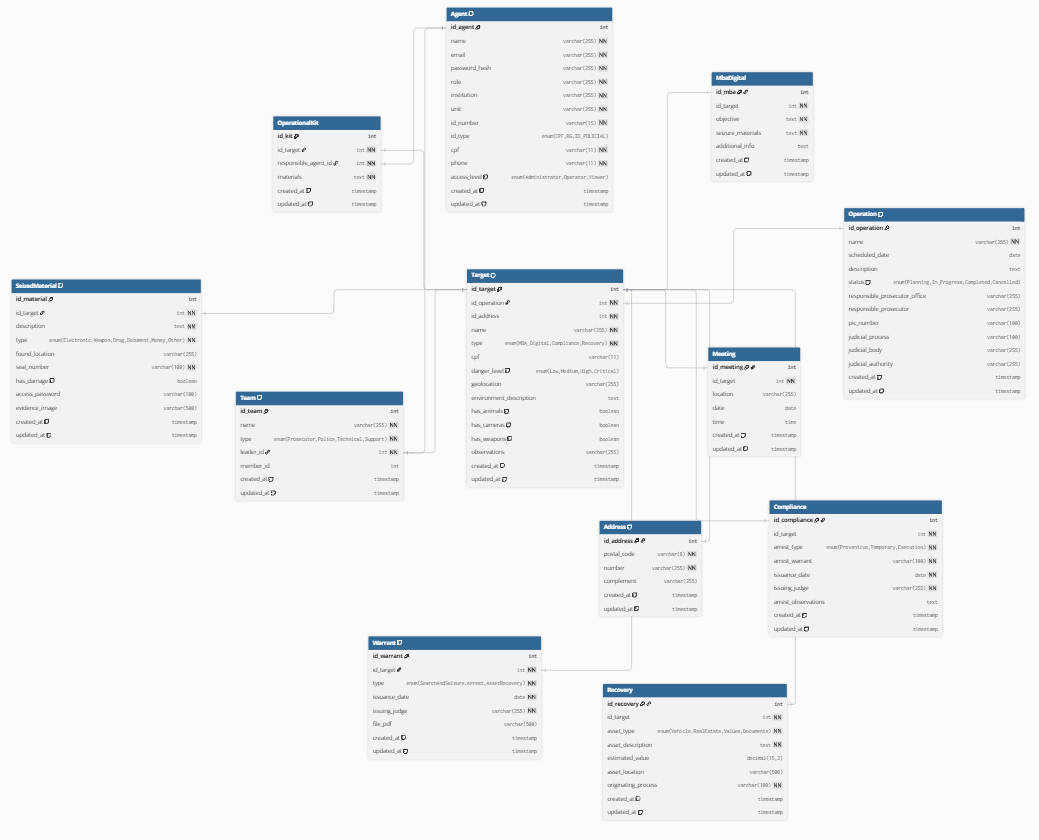
\includegraphics[width=1\linewidth]{conteudo//2 - ages I//conteudo//figures//banco_de_dados.png}
    \caption{Modelo do banco relacional}
    Fonte: Adaptado de \textcites{wiki-vincula}
    \label{fig:modelo-banco}
  \end{figure}

\newpage
\subsection{Arquitetura Utilizada}
  A arquitetura do projeto Operações GAECO foi projetada para ser executada na nuvem da \ac{aws} \cite{aws}, utilizando uma combinação de serviços gerenciados e um ambiente containerizado para garantir eficiência e automação no ciclo de desenvolvimento. A \autoref{fig:diagrama-deploy} mostra o diagrama de Deploy na \acs{aws}.

  \begin{figure}[H]
    \centering
    \small
    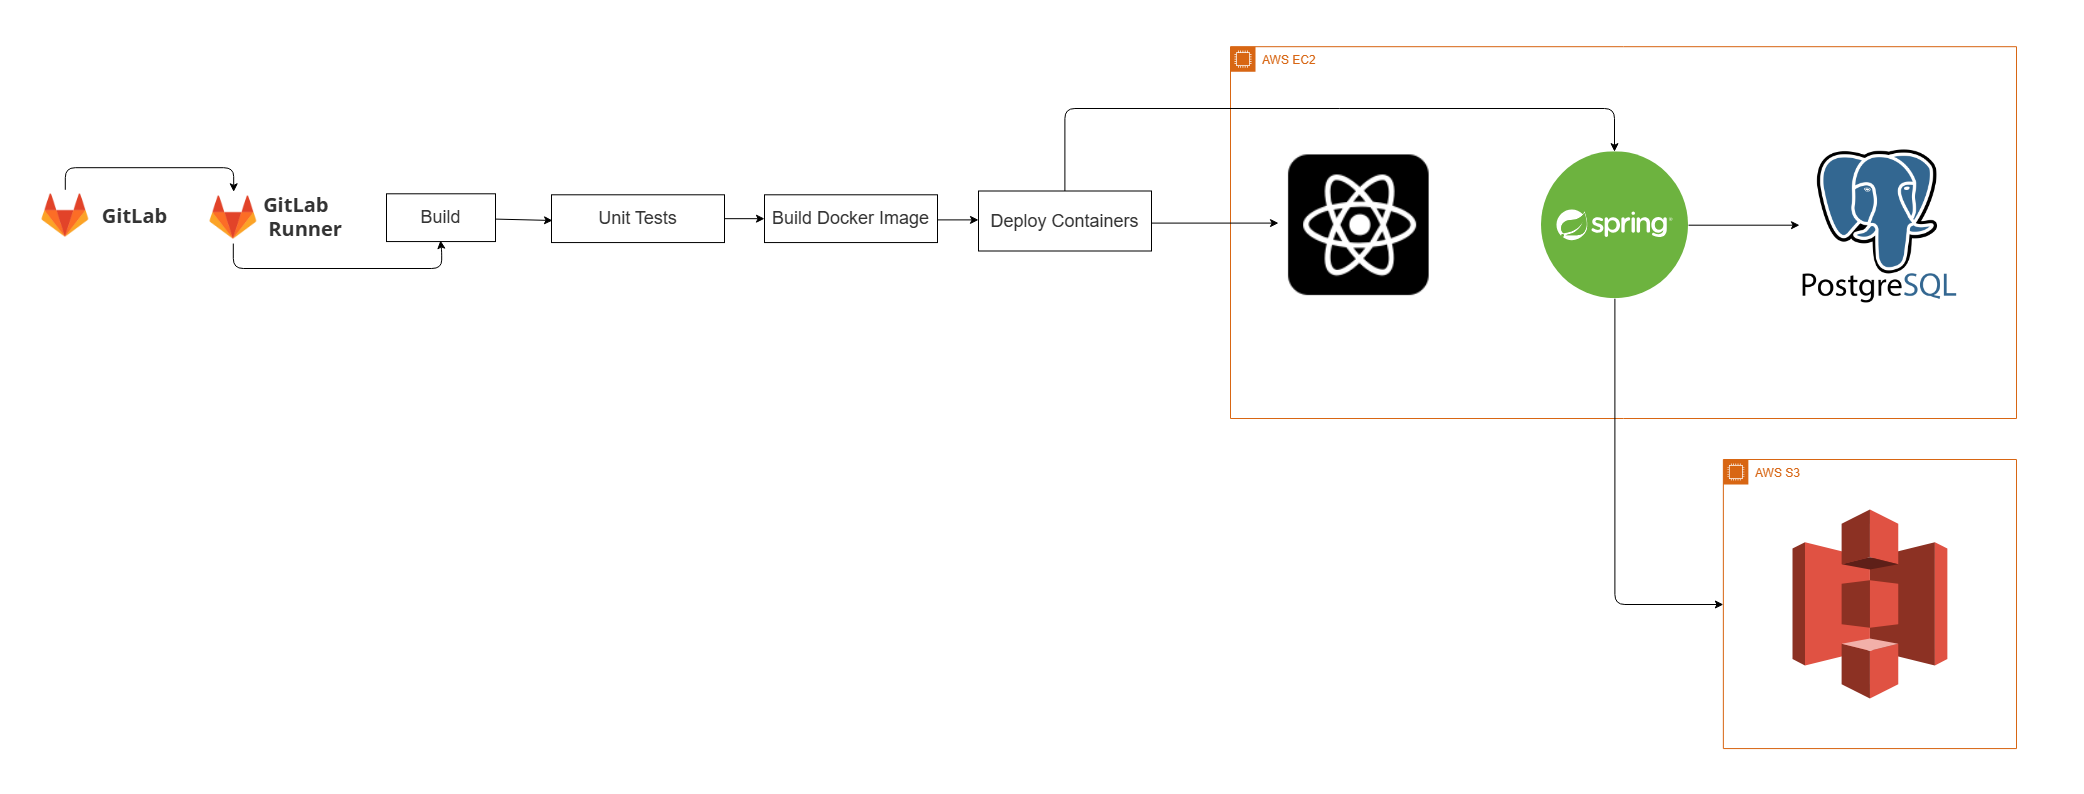
\includegraphics[width=1\linewidth]{conteudo//2 - ages I//conteudo//figures//Diagrama_de_Deploy.png}
    \caption{Diagrama de Deploy}
    Fonte: Adaptado de \textcites{wiki-Operacoes GAECO}
    \label{fig:diagrama-deploy}
  \end{figure}

  Conforme ilustrado pelo diagrama da \autoref{fig:diagrama-deploy}, a arquitetura da solução segue um fluxo claro e desacoplado. A interface com o usuário, hospedada no AWS Amplify \cite{amplify}, consome uma API backend em Java \cite{java} com Spring Boot. Esta API, juntamente com o banco de dados PostgreSQL, opera de forma containerizada com Docker \cite{docker} em uma instância Amazon EC2 \cite{ec2}. O sistema é complementado pelo Amazon S3 \cite{s3}, responsável pelo armazenamento de arquivos.

\subsection{Protótipos das Telas Desenvolvidas}
  Os protótipos para as telas centrais da aplicação foram desenvolvidos utilizando a ferramenta Figma \cite{figma}. O manual de identidade visual do \acs{mprs} foi usado como referência para cores, estilo e logomarcas. 
  
  Algumas das telas são: Tela de Autenticação (\autoref{fig:tela-login}), Tela de Listagem de Operações (\autoref{fig:tela-operacoes}) e Tela do Caso (\autoref{fig:tela-alvos}).

  As demais telas estão disponíveis no Figma do projeto:
  
  \url{https://www.figma.com/design/eDNVyvDaNWyvONdiL053ff/Opera%C3%A7oes-GAECO}

  \begin{figure}[H]
    \centering
    \small
    
\includegraphics[width=0.4\linewidth]{conteudo//2 - ages I//conteudo//figures//tela-login.png}
    \caption{Tela de Autenticação}
    Fonte: Adaptado de \textcites{figma-Operacoes GAECO}
    \label{fig:tela-login}
  \end{figure}

  \begin{figure}[H]
    \centering
    \small
    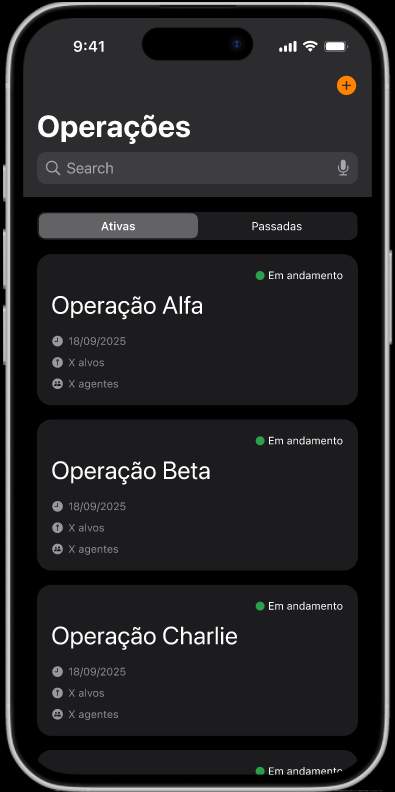
\includegraphics[width=0.4\linewidth]{conteudo//2 - ages I//conteudo//figures//tela-operacoes.png}
    \caption{Tela de Listagem de Operações}
    Fonte: Adaptado de \textcites{figma-Operacoes GAECO}
    \label{fig:tela-operacoes}
  \end{figure}

  \begin{figure}[H]
    \centering
    \small
    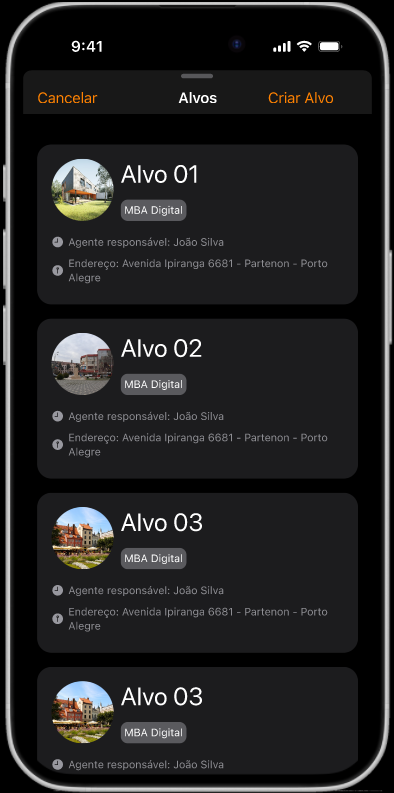
\includegraphics[width=0.4\linewidth]{conteudo//2 - ages I//conteudo//figures//tela-alvos.png}
    \caption{Tela de Listagem de Alvos}
    Fonte: Adaptado de \textcites{figma-Operacoes GAECO}
    \label{fig:tela-alvos}
  \end{figure}

\subsection{Tecnologias Utilizadas}
  O projeto é construido utilizando quatro tecnologias principais, sendo elas o React Native \cite{react} com Expo \cite{nextjs} e a linguagem TypeScript \cite{typescript} para o frontend, o Spring Boot \cite{fastapi}, com a linguagem Java para o backend, PostgreSQL para o banco relacional.
  
  O Spring Boot foi escolhido por sua facilidade de configuração, suporte a microserviços, integração com diversos bancos de dados e ecossistema rico para desenvolvimento de APIs REST.

  No backend, logo de início, decidimos que este projeto utilizaria Java 21, uma linguagem robusta, orientada a objetos e amplamente utilizada para aplicações corporativas.

  O gerenciamento de tarefas, o planejamento das sprints e o controle do backlog são realizados na plataforma ClickUp. O controle de versão é feito com Git, hospedado no servidor da \acs{ages}. Todo o ambiente de desenvolvimento é containerizado com Docker.
\section[Atividades Desempenhadas Pelo Aluno no Projeto]{Atividades Desempenhadas Pelo Aluno no Projeto}

\subsection{Sprint 0}

Durante a Sprint 0, o time focou no planejamento e na prototipagem das interfaces da plataforma Vincula. Enquanto os colegas \ac{ages} II desenhavam o modelo inicial do banco de dados e os \ac{ages} III e IV definiam a arquitetura, minha contribuição inicial foi na colaboração com os mockups das telas essenciais no Figma, como as de Home, Login e a de Visualização de Casos.

Por ser minha primeira experiência na \ac{ages}, após a fase inicial de prototipagem, encontrei um desafio em identificar os próximos passos e reconheço que faltou proatividade da minha parte para buscar novas tarefas. Decidi, então, focar em estudar as tecnologias para as futuras sprints de desenvolvimento do backend.

Para isso, desenvolvi um projeto de estudo prático com FastAPI, implementando funcionalidades de cadastro de usuários, login e autenticação com \ac{jwt}, o que me deu uma base sólida para as tarefas que viriam a seguir. Adicionalmente, para entender a complexidade dos dados que iremos manipular, criei scripts com a biblioteca Pandas para fazer uma análise exploratória nos arquivos de exemplo disponibilizados pelos stakeholders provenientes do \ac{simba} e do \ac{sittel}, o que me permitiu entender na prática como os vínculos se formam.

A sprint terminou com a apresentação dos mockups e das User Stories planejadas para a Sprint 1 aos stakeholders. Posteriormente, a retrospectiva da Sprint 0 foi uma experiência de grande importância para meu aprendizado, pois nela pude esclarecer minhas dúvidas e alinhar com os colegas AGES IV questões sobre a comunicação e responsabilidades. A conversa me acalmou quanto às incertezas sobre a organização de tarefas, pois entendi que a natureza da Sprint 0 é realmente mais fluida e exploratória, sem uma definição de atividades individuais tão rígida como nas sprints de desenvolvimento.

A lição mais importante desta sprint foi a importância da comunicação e da proatividade. Aprendi que é minha responsabilidade buscar ativamente o alinhamento com a equipe e pedir direcionamento. Ao final da Sprint 0, sinti-me tecnicamente mais preparado para as tarefas de backend e, principalmente, mais ciente da postura colaborativa que o projeto exige para as próximas etapas.
\subsection{Sprint 1}

Com o planejamento concluído, a Sprint 1 marcou o início efetivo do desenvolvimento da plataforma. Fui responsável por duas tarefas principais que abrangeram tanto o backend quanto o frontend, permitindo-me aplicar os conhecimentos adquiridos na fase de estudos. No backend, implementei o endpoint para listagem de casos (`GET /cases`), que incluía a lógica de paginação, filtragem dinâmica e a proteção de rota via token de autenticação. Este trabalho exigiu colaboração com o colega Bryan Leandro, para integrar a funcionalidade com o sistema de login, e foi refinado com base no feedback dos colegas Felipe Cardona e Gabriel Belmonte.

No frontend, desenvolvi um componente de `Input` genérico e reutilizável com React e Material-UI \cite{materialui}, seguindo as especificações do Figma, os princípios de componentes do NextJs e alinhando as decisões de implementação com as colega Lara Kunrath e Carolina Ferreira. Além das minhas tarefas designadas, procurei manter uma postura colaborativa, auxiliando os colegas Rodrigo Schmitt e Gabriel Pinho com suas tarefas.

O principal desafio desta sprint não foi técnico, mas sim de processo e comunicação dentro da equipe. Observei que a falta de uma sincronia técnica inicial entre desenvolvedores trabalhando em partes interconectadas do sistema levou a inconsistências no padrão de código, o que gerou retrabalho no final da sprint. Essa experiência reforçou a lição da sprint anterior sobre a importância da proatividade.

Aprendi que, para garantir a consistência e a qualidade da base de código, a comunicação técnica no início do desenvolvimento de uma tarefa é tão crucial quanto o code review no final. Ao final da Sprint 1, ambas as minhas tarefas foram concluídas e integradas com sucesso. Sinto que solidifiquei meu conhecimento prático em FastAPI e NextJs e, mais importante, obtive uma visão mais clara de como minha comunicação proativa pode contribuir diretamente para a qualidade técnica e a eficiência de toda a equipe.
% \subsection{Sprint 2}

Durante o andamento da Sprint 2, foram divididas novas squads, e suas respectivas tarefas, eu e minha squad recebemos a responsabilidade de desenvolver a tela de contatos, a qual necessitava de um card de contatos, uma tela de adição de contatos e um endpoint no backend para que fosse possível obter os contatos do usuário autenticado.

Como estava em época de provas, resolvi escolher a task que acreditava ter mais domínio sobre, sendo ela o desenvolvimento do card de contatos, já que na sprint passada havia passado grande parte do tempo desenvolvendo em Flutter.

O desenvolvimento do card foi uma tarefa relativamente simples, sendo necesário apenas o desenvolvimento de um botão a parte, para que fosse possível manter a borda circular do card. A parte mais complicada foi encontrar uma maneira de possibilitar que o card fosse alterado de leitura para edição, para ser possivel implementar o modo de edição dos contatos.

No fim da sprint quase tudo deu certo, faltando apenas a validação dos dados inseridos na tela de criação de novos contatos, porém, apesar desse problema, a cliente, novamente, se mostrou muito satisfeita com o progresso que o time teve durante a sprint 2. Infelizmente, acabamos ficando, novamente com débito técnico para entregar na Sprint seguinte, porém conseguimos resolver o débito técnico que havia sido repassado da Sprint 1.
% \subsection{Sprint 3}

No inicio da Sprint 3 foram divididas as squads e suas respectivas tarefas novamente, dessa vez, eu e minha squad ficamos incumbidos da criação do endpoint e dados mockados das telas e dicas do aplicativo.

Esta sprint ocorreu em uma época mais tranquila em relação à faculdade, possibilitando um maior empenho no projeto. Como teria mais tempo para trabalhar no projeto achei que seria uma boa ideia tentar algo que ainda não havia feito, por isso acabei decidindo fazer a rota para recuperar as dicas.

O trabalho feito no endpoint foi bem interesante e desafiador, já que era algo completamente diferente do que eu havia feito até o momento, mas foi possível completar a task sem grandes dificuldades.

Durante o andamento da sprint tivemos alguns problemas originados de algumas \ac{us} mal planejadas. Após as correções necesárias, tanto no código ja desenvolvido, quanto nas \ac{us}, as tarefas atribuídas a nossa squad foram finalizadas, restando ainda tempo para o fim da Sprint.

Por conta de termos finalizado nossa \ac{us} com antecedência, resolvi ir além e fazer os testes unitários do endpoint implementado e, também, organizar os dados mockados em diferentes arquivos json, mantendo assim, uma boa organização no projeto.

Embora tenha feito algo novo nessa sprint, tudo ocorreu de acordo com o esperado e sem problemas na entrega, tendo, novamente, uma cliente muito feliz com os resultados obtidos pelo time durante a terceira sprint. Felizmente, nessa Sprint conseguimos resolver todos os débitos técnicos repassados e, também, conseguimos finalizar todas tarefas planejadas, além de fazer um crédito técnico por ter realizado alguns dos testes unitários que seriam feitos em Sprints futuras.
% \subsection{Sprint 4}

Novamente, como nas sprints passadas, no início da Sprint 4 foram divididas 
as tasks e as squads, dessa vez fui atribuído a squad Água, que estava responsável 
pela seleção de uma \ac{api} de notícias, integração da \ac{api} com 
o programa, criação do carrossel de notícias e do card de notícias.

Nessa última sprint retornei para o desenvolvimento do front end do projeto, 
pois foi a área que mais me interessou e que eu mais estudei. Após esta decisão fiquei 
responsável pela criação do card de notícias, que deveria seguir o padrão feito no 
\cite{figma}. 

A produção do card não foi algo que demonstrou muita dificuldade, porém eu 
ainda não havia trabalhado com imagens, portanto precisei pesquisar e descobrir 
como faria para carregar uma imagem a partir de uma \ac{url}, assim como aprender a aplicar um gradiente de opacidade ao longo da imagem.

Quando terminei o card notei que a pipeline estava dando erro, porém não 
parecia ser um problema vindo do meu código, por isso, fui procurar a fonte do 
erro e descobri que ela estava excedendo o tempo máximo de execução do script. 
Informei aos colegas que conseguiriam lidar com o problema e aguardei a correção.

Após a correção da pipeline, quando juntamos tudo que havia sido feito, 
notamos que a \ac{api} que havíamos escolhido tinha um limite de 5 chamadas por dia, 
assim, foi necessário procurar outra \ac{api} que nos entregasse o que precisávamos. Por 
fim, foi necessário mockar os dados, já que estávamos nos aproximando da data de 
entrega e não havíamos encontrado uma \ac{api} que entregasse o que precisávamos. 

Ao fim da Sprint, embora tenhamos encontrado alguns problemas, tudo foi 
entregue. Tivemos um feedback muito positivo vindo da cliente, que estava muito 
contente com os resultados que obtivemos ao longo do projeto. 
%\section[Conclusão]{Conclusão}
  %\chapter[AGES II --- “NOME DO PROJETO XXXX”]{AGES II --- “NOME DO PROJETO XXXX”}

\section[Introdução]{Introdução}

O projeto Sow Good foi pensado e apresentado para nós pelos stakeholders Dr. Ricardo Reichenbach e Dra. Valéria Cristina Artico. O mesmo foi supervisionado pelo professor orientador Rafael Chanin.

O objetivo principal do projeto é criar um aplicativo que melhore e facilite a comunicação entre pediatra e responsáveis do paciente e forneça informações confiáveis para os guardiões da criança.

\begin{figure}[H]
    \centering
    \small
    \caption{Time Sow Good}
    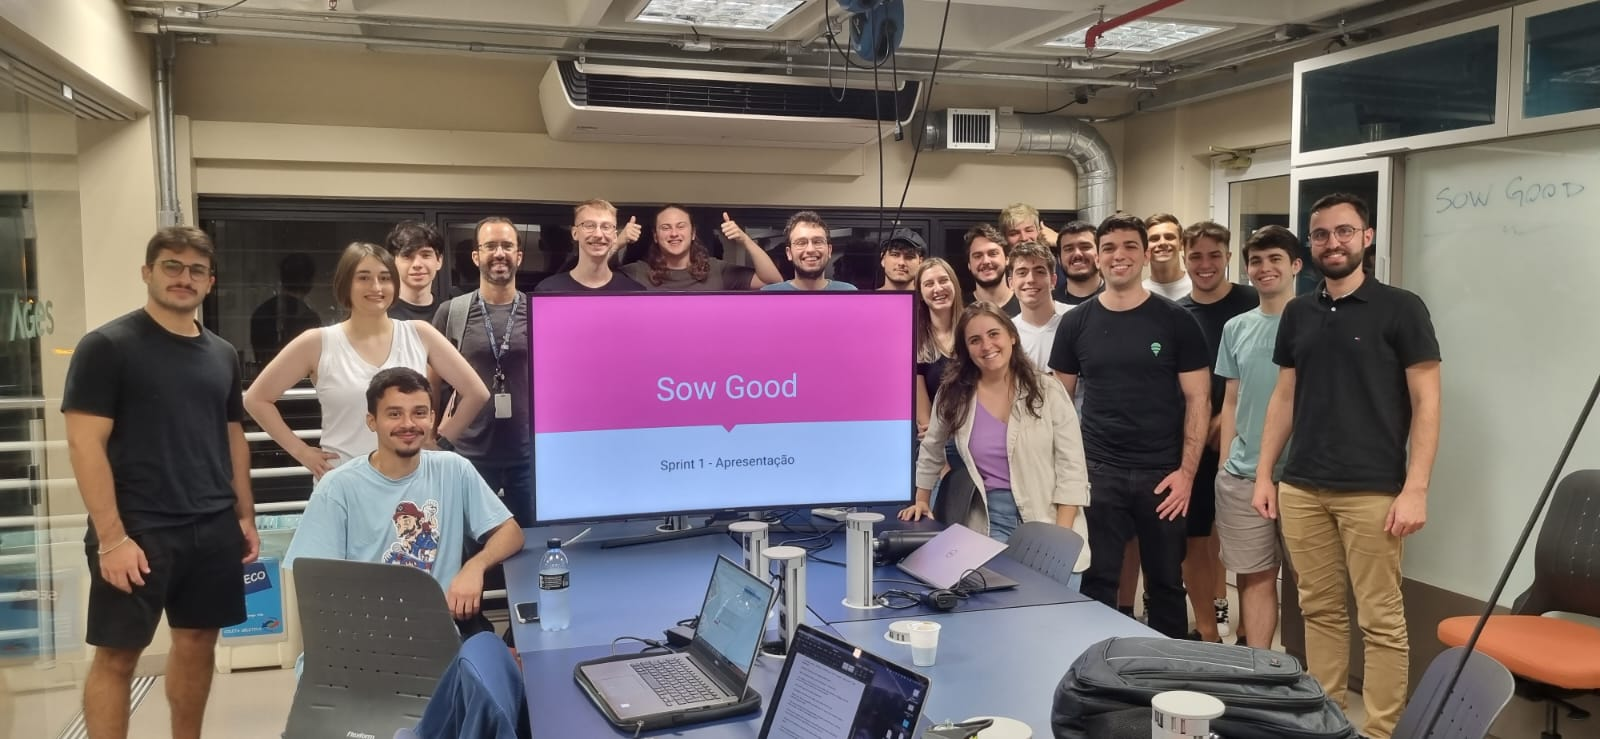
\includegraphics[width=1\linewidth]{conteudo//3 - ages II//conteudo//figures//foto-time.png}
    Fonte: https://tools.ages.pucrs.br/sow-good/wiki/-/wikis/home
\end{figure}
\section[Desenvolvimento do Projeto]{Desenvolvimento do Projeto}

\subsection{Repositório do Código Fonte do Projeto}
Para este projeto foram utilizados dois repositórios para código e um para a wiki, todos foram mantidos no GitLab da AGES. A separação dos repositórios de código foi feita em frontend, o qual utiliza a tecnologia Flutter\cite{flutter}, usando a linguagem Dart\cite{dart} e backend, que utiliza as tecnologias NodeJs\cite{nodejs} e ExpressJs\cite{expressjs}, usando a linguagem JavaScript\cite{javascript} e TypeScript\cite{typescript}

\begin{itemize}
  \item Sow Good wiki: https://tools.ages.pucrs.br/sow-good/wiki/-/wikis/home
  \item Sow Good frontend: https://tools.ages.pucrs.br/sow-good/sow-good-frontend
  \item Sow Good backend: https://tools.ages.pucrs.br/sow-good/sow-good-backend
\end{itemize}

\subsection{Banco de Dados Utilizado}
Inicialmente foi pensado em utilizar um banco de dados relacional para a realização do projeto por conta da sua simplicidade e ser conhecido por todos integrantes da equipe, porém, com o andamento da Sprint 0 foi decidido que seria melhor utilizar um dos bancos de dados disponibilizados pelo Firebase, dado que estaríamos utilizando o Firebase Authentication, um produto que iria fazer a criação e autenticação dos usuários, além de guardar informações críticas de forma segura, o que iria nos facilitar na parte de cadastro e login dos usuários.

Dentre as opções diponibilizadas pelo Firebase, acabamos escolhendo o Firestore\cite{firestore} Database que é o banco de dados não relacional disponibilizado pela Firebase\cite{firebase}. Uma outra opção seria utilizar o Realtime Database\cite{realtimedb}, que também utiliza o esquema não relacional, porém, alguns integrantes da equipe ja possuíam experiência com o Firestore\cite{firestore}, sendo esse, o motivo pelo qual escolhemos utilizá-lo.

\begin{figure}[H]
    \centering
    \small
    \caption{Esquema Conceitual Banco de Dados Sow Good}
    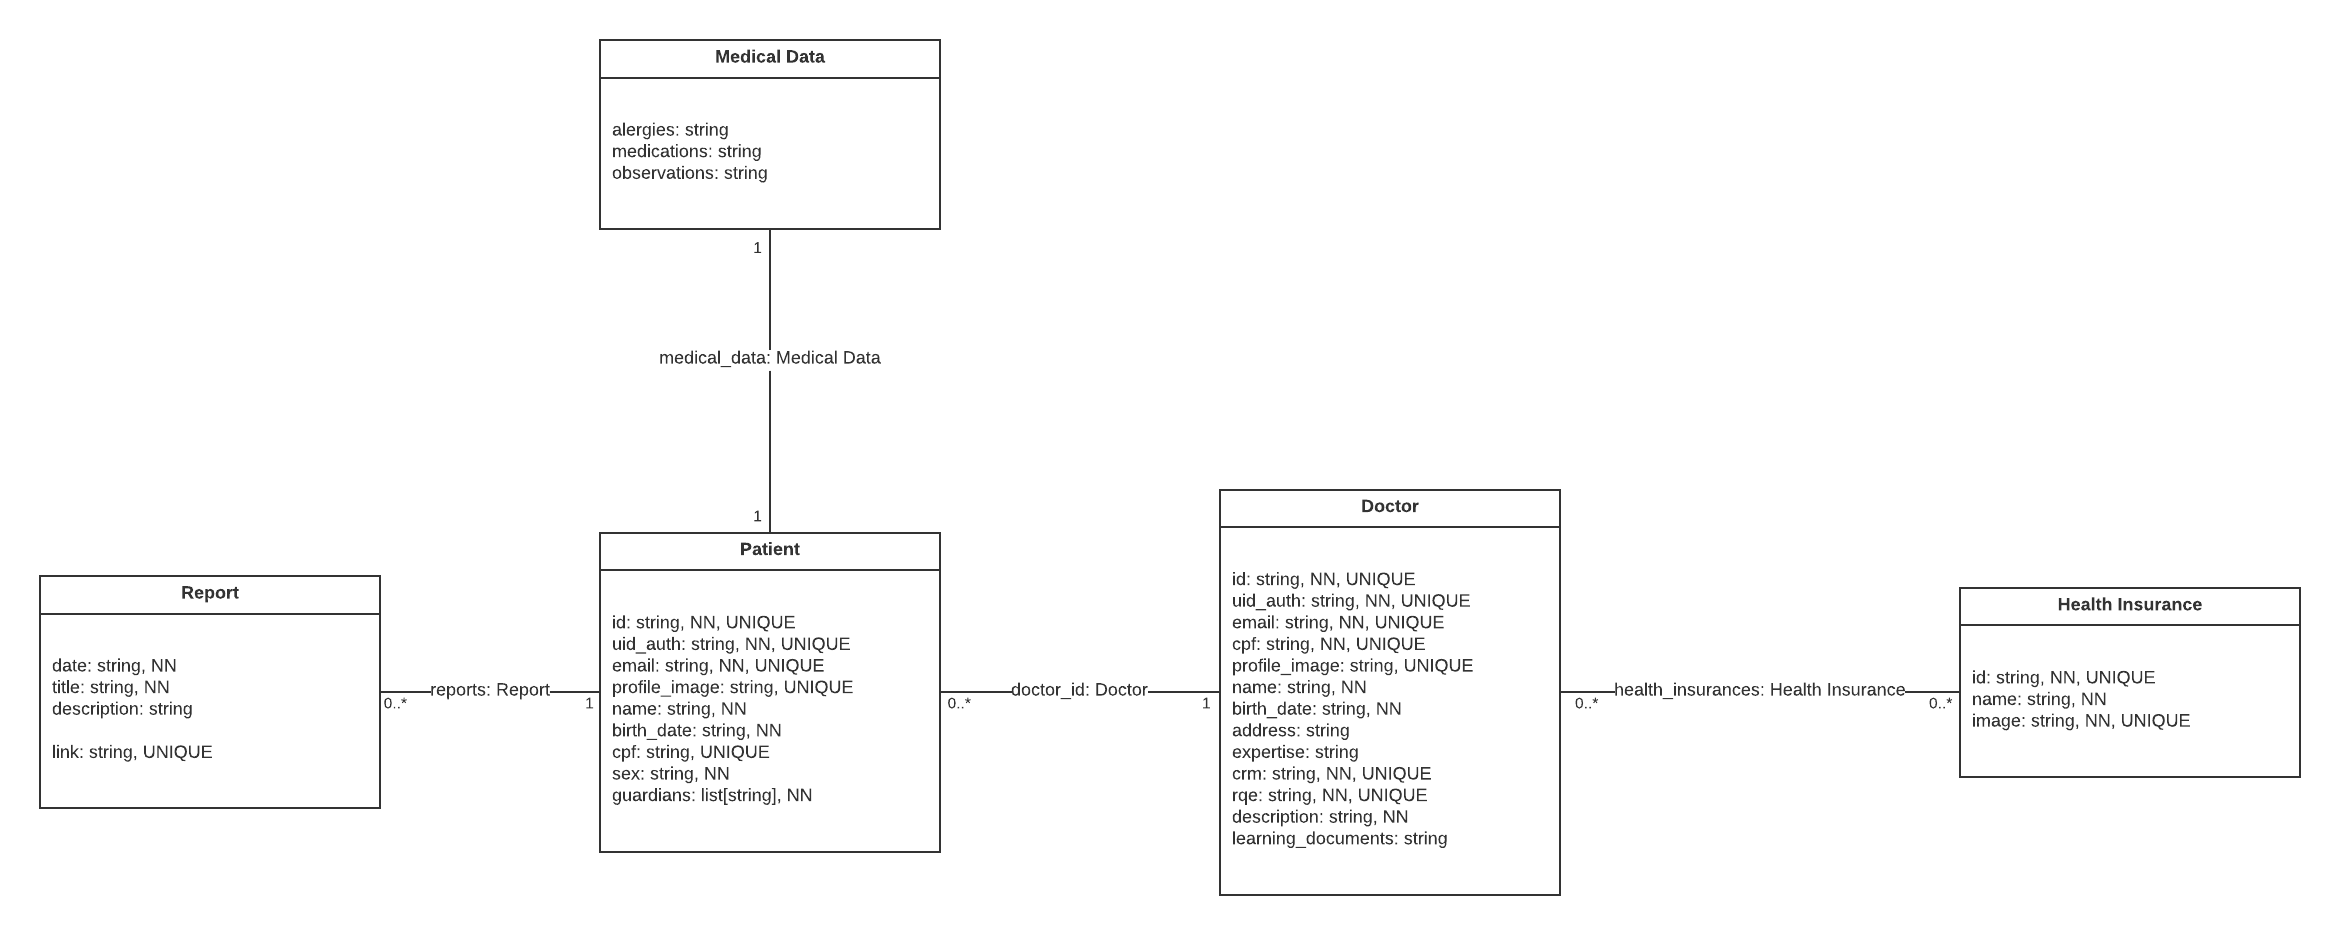
\includegraphics[width=1\linewidth]{conteudo//3 - ages II//conteudo//figures//bd-conceitual.png}
    Fonte: https://tools.ages.pucrs.br/sow-good/wiki/-/wikis/banco\_dados
\end{figure}

\subsection{Arquitetura Utilizada}
A arquitetura, assim como foi na AGES I, segue o modelo cliente-servidor 
que consiste em três partes principais, o banco de dados, onde são guardados todos 
dados necessários para o funcionamento correto do sistema, o servidor que conecta 
o cliente ao banco de dados, fazendo toda a transformação do tipo de dados e 
tratamento necessários, assim devolvendo uma informação utilizável pelo cliente que 
é a última parte do modelo e o cliente, que é responsável por apresentar as informações recebidas do servidor através de uma interface gráfica de fácil utilização.

\begin{figure}[H]
    \centering
    \small
    \caption{Arquitetura Geral Sow Good}
    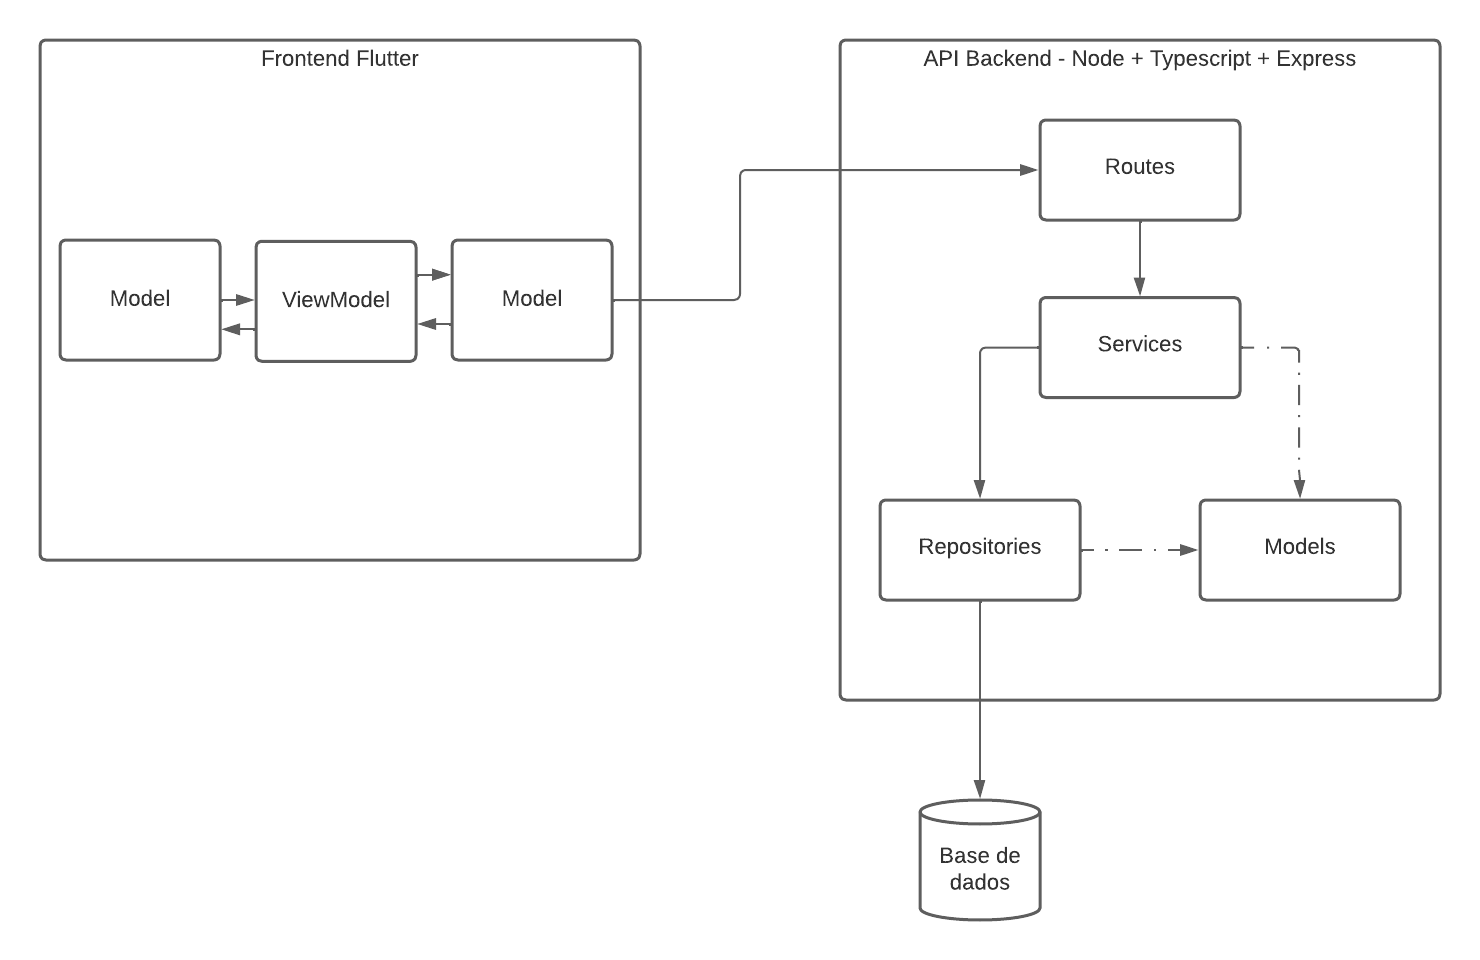
\includegraphics[width=1\linewidth]{conteudo//3 - ages II//conteudo//figures//arquitetura-geral.png}
    Fonte: https://tools.ages.pucrs.br/sow-good/wiki/-/wikis/arquitetura
\end{figure}

\subsection{Protótipos das Telas Desenvolvidas}
Dado que inicialmente o projeto ainda não possuía uma identidade visual bem 
definida, seguimos padrões de design mais comumente utilizados, como, por exemplo, componentes mais arredondados, um bom contraste de cores para que o aplicativo pudesse ser utilizado 
por pessoas com problemas visuais com facilidade e tamanho e cor de letras para 
permitir uma leitura fácil. Para produzir os protótipos foi usada a plataforma Figma\cite{figma}, que permite que várias pessoas desenvolvam simultaneamente, diminuindo a quantidade de retrabalho e aumentando a eficiênciado time.

\begin{itemize}
  \item https://tools.ages.pucrs.br/sow-good/wiki/-/wikis/mockups
\end{itemize}

\subsection{Tecnologias Utilizadas}

O projeto foi construído utilizando cinco tecnologias diferentes, sendo elas o 
Flutter\cite{flutter} com a linguagem Dart\cite{dart} para o frontend, o NodeJs\cite{nodejs} para o backend utilizando ExpressJs\cite{expressjs} para lidar com os diferentes endpoints existentes na \ac{api}, o Firebase Authentication\cite{firebaseauth} para lidar com cadastro e login de usuários e Firestore\cite{firestore} como banco de dados.

A escolha do Flutter\cite{flutter} para o frontend foi feita pois é uma das tecnologias que 
permite o desenvolvimento de aplicações para Android, IOS e Web em uma única 
linguagem, diminuindo, assim, o estudo e trabalho necessário para o desenvolvimento 
do projeto.

Para o backend foi escolhido o NodeJs\cite{nodejs} por ser uma tecnologia muito utilizada 
atualmente e por diversos integrantes da equipe possuir um conhecimento prévio 
acerca da ferramenta, assim, podendo ajudar quem estiver tendo problemas. O uso 
do ExpressJs\cite{expressjs} foi feito para que pudesse haver uma maneira mais organizada de definir cada endpoint existente na nossa \ac{api}. 

O Firebase Authentication\cite{firebaseauth} foi utilizado para facilitar e diminuir o trabalho 
necessário para a implementação de um sistema de autenticação, permitindo que a equipe foque em outros pontos importantes da aplicação. 

O Firestore\cite{firestore}, assim como o NodeJs\cite{nodejs}, foi escolhido por alguns 
integrantes da equipe já possuir conhecimento prévio acerca da ferramenta, e, 
também, por ser, assim como o Firebase Authentication\cite{firebaseauth} e o Flutter\cite{flutter}, uma tecnologia desenvolvida pela Google\cite{google}, ou seja, elas possuem grande compatibilidade entre sí.
\section[Atividades Desempenhadas Pelo Aluno no Projeto]{Atividades Desempenhadas Pelo Aluno no Projeto}

\subsection{Sprint 0}

Durante o andamento da Sprint 0, foi definido, junto com os stakeholders, um 
padrão para ser seguido no design do projeto, porém, como foi descrito anteriormente, 
a aplicação ainda não possuía uma identidade visual bem definida, por isso, alguns 
parâmetros foram estabelecidos com eles, como, por exemplo, evitar a utilização de tons pasteis, que são cores com tons mais pálidos. Também foi definido que seria 
melhorar utilizar componentes mais arredondados, para serem mais atrativos e amigáveis para os possíveis usuários.

Nessa etapa não vimos necessidade de fazer divisão de tasks por squads, por isso, combinamos o que cada um iria fazer por afinidade com a ferramenta Figma\cite{figma}. Foi delegado para mim a atividade de projetar a tela de apresentar o QR Code do médico, que seria a maneira como os pacientes iriam conectar a sua conta com a do médico. Acabei desenvolvendo diversos protótipos até chegar em um que achei que encaixaria bem com a identidade visual que estava se formando.

Além do desenvolvimento dessa tela, também auxiliei outros colegas no desenvolvimento do 
protótipo deles, fiz a revisão para que todas as telas estivessem usando os 
componentes desenvolvidos no style guide e me certifiquei que a navegação dos 
mockups estava correta e funcional para a apresentação para os stakeholders.

Além de desenvolver os mockups, eu criei um esquema conceitual para o 
banco de dados. Para isso utilizei a ferramenta LucidChart\cite{lucidchart}, que permite a criação de diagramas, fluxos e até mesmo mockups de forma fácil e rápida.

Apesar de grande parte dos integrantes da equipe não possuir experiência com 
o Figma\cite{figma}, tudo ocorreu de acordo com o esperado e os stakeholders se mostraram 
bem satisfeitos com o resultado que obtivemos, porém indicaram algumas alterações 
que gostariam que fossem aplicadas aos protótipos que foram feitos assim que 
possível.
\subsection{Sprint 1}

No começo da Sprint 1 foram divididas as squads, para que todos pudessem trabalhar e experimentar todas as tecnologias utilizadas no projeto, todas squads possuíam tasks, tanto de backend, quanto de frontend. Após a divisão dos integrantes da equipe entre as squads eu fui designado para a squad 2, que tinha a responsabilidade de desenvolver o cadastro do paciente.

Dentro da minha squad eu fiquei responsável por desenvolver a tela para adicionar os responsáveis do paciente e de criar o endpoint da \ac{api} que iria cadastrar a conta no 
Firebase Authentication\cite{firebaseauth} e salvar os dados do paciente no banco de dados.

Por já possuir uma experiência prévia com Flutter\cite{flutter} consegui desenvolver a tela sem muitos problemas. Durante o desenvolvimento da tela notei que seria melhor a criação de um componente especial para aceitar a escrita do usuário já que o componente existente estava recebendo muitas variáveis, tornando-o muito complexo para o entendimento.

Para o desenvolvimento do endpoint de cadastro foi necessário um pouco de estudo, já que nunca havia utilizado ExpressJs\cite{expressjs} para lidar com as rotas. Nessa parte tive um pouco mais de dificuldade, pois não possuía tanta experiência quanto em Flutter\cite{flutter}, porém consegui desenvolver um endpoint funcional. Ao longo da Sprint 1 ela precisou ser alterada para atender algumas alterações que estavam sendo realizadas na arquitetura do projeto, porém foi finalizada a tempo para a entrega. 

Além de realizar minhas tarefas, ajudei, também, vários \ac{ages} I com suas respectivas tasks, ensinando qual nomenclatura deveria ser utilizada, em quais pastas cada componente e tela deveria estar, e, também ajudando a desenvolver e finalizar as tasks. 

Ao fim dessa sprint não conseguimos entregar tudo que estava planejado para os clientes, ficando assim, com alguns débitos técnicos para a próxima sprint, porém, apesar dos problemas, eles gostaram bastante do que foi feito. Acredito fortemente que esse débito técnico ocorreu por ainda estarmos nos conhecendo como time o que diminui a produtividade da equipe como um todo.
\subsection{Sprint 2}

Com o início da segunda sprint dividimos, novamente, o time em 3 squads diferentes, porém foi alterada a dinâmica de todas squads trabalharem tanto com backend quanto com frontend, pois notamos que seria melhor que os integrantes pudessem se manter focados em uma tecnologia durante todo o projeto e seguimos esse pensamento o máximo possível.

Após a divisão das squads fui designado para a squad 3, que, em geral, estaria responsável da correção de bugs, porém acabei ficando responsável por desenvolver o Swagger\cite{swagger} do projeto por já ter experiência com a ferramenta. Consegui finalizar a tarefa com facilidade grande parte do que precisava ser feito. Além das funcionalidade visuais do Swagger\cite{swagger}, também queríamos adicionar a capacidade de testar os endpoints utilizando a \ac{ui}, para isso, foi necessário fazer um estudo acerca dessa utilidade.

Após finalizar minha task, resolvi auxiliar meu colegas com o redesenvolvimento de alguns endpoints para que apenas usuários que tivessem uma conta e estivessem autenticados conseguissem consumir algumas partes da \ac{api}.

Além de tarefas de desenvolvimento de código, estava constantemente auxiliando outros colegas da AGES com tasks, tanto de back, quanto de frontend, porém nessa sprint contribui majoritariamente com tarefas de backend, por estar altamente atrelado ao que eu havia desenvolvido na sprint.

Infelizmente, ao final da sprint, novamente, não conseguimos entregar tudo que foi planejado, porém alguns pontos que eram possíveis causadores disso foram observados e apontados, para que pudessem ser corrigidos o mais rápido possível. Acredito que a entrega da sprint 2 não tenha sido muito boa da perspectiva dos clientes, pois, apesar do backend da aplicação ter sido completamente entregue, a parte visual, ou seja, o frontend, estava com diversos débitos técnicos. 
\subsection{Sprint 3}

Com o início da terceira sprint, o time foi separado em equipes de 5 pessoas, novamente, buscamos manter a forma de organizar as squads focadas em áreas específicas, pois essa técnica mostrou um melhor resultado do que as squads terem responsabilidades tanto no backend, quanto no frontend.

Nessa sprint voltei a ser um membro da squad 2 e ficamos responsáveis por desenvolver algumas telas e componentes do fluxo dos médicos. A parte definida para mim inicialmente foi desenvolver a tela de menu do médico, porém notamos que essa sprint teria uma duração bem reduzida, de cerca de 2 semanas, por isso, acabei reorganizando as tasks e peguei tarefas com uma alta prioridade por ter mais experiência e tempo livre para realizá-las no período determinado. 

Com isso, acabei ficando responsável por desenvolver o componente de perfil do médico, no qual seria apresentado sua imagem, seu nome, endereço do consultório, especialização e descrição. Comecei a trabalhar o mais cedo possível para que entregasse dentro do prazo esperado, porém a task se mostrou mais difícil de finalizar do que o esperado, pois muitas outras tarefas menores estavam “escondidas” dentro dela, como por exemplo a criação de uma modal para selecionar os convênios aceitos pelo médico e as variações de visualização e de edição do componente e, por isso, o prazo acabou sendo excedido em um dia.

Ao finalizar a criação do componente me mostrei disponível para auxiliar os colegas em suas respectivas tasks, auxiliando, também, colegas de outras squads que estavam com suas tarefas trancadas e não sabiam como avançar.

Apesar de nossos esforços para terminar o que foi combinado no período da terceira sprint, não conseguimos entregar grande parte do que era esperado, além disso, o que foi entregue possuía vários problemas a serem corrigidos, por isso, a próxima e última sprint teria que ser muito bem planejada e organizada para que o projeto seja finalizado e entregue de forma completa e satisfatória para os cliente.
\subsection{Sprint 4}

Após a curta duração da sprint 3 e a grande quantidade de débito técnico e correções para serem feitas, decidimos manter as mesmas squads para a quarta sprint, o que iria economizar tempo e permitir usá-lo para desenvolvimento. Por eu ser o integrante com mais experiência em desenvolvimento em Flutter\cite{flutter} e Dart\cite{dart}, as tarefas de criação de novas features foram designadas para minha squad, juntamente com algumas de correção de bugs.

Com isso, fiquei designado de desenvolver o QR Code que seria usado para atrelar um médico a um paciente. Essa task não se mostrou muito difícil de completar, dado que já havia trabalhado com modal na sprint passada e para a geração de um QR Code existem diversas \ac{api}s que poderiam ser utilizadas. Como consegui terminar minha tarefa rapidamente, procurei auxiliar o máximo de colegas possível sabendo que teríamos muito o que fazer nessa última sprint.

Comecei conversando com o colega responsável por desenvolver a tela para ler o QR Code para conectar um médico a um paciente, porém ele comunicou que acreditava estar fazendo um bom progresso sozinho, então fui procurar outras pessoas para auxiliar. 

Acabei auxiliando uma colega que estava responsável pela tela de cadastro. Essa tela havia sido desenvolvida na última sprint, porém apresentava diversos problemas, por isso, optei por indicar que seria uma boa ideia começar a tela do zero, por haver uma grande quantidade de problemas na estruturação do código, o que acarretaria outros problemas posteriormente. Essa correção levou um tempo para conseguir ser feita, dado que algumas outras utilidades da aplicação haviam sido alteradas, como, por exemplo, os validadores que estavam sendo usados nas áreas de escrita, por isso, tivemos que estudar o código e entender como estavam sendo usados e, assim, alterar a tela de acordo.

O último fim de semana antes da entrega foi extremamente corrido, pois muitas correções ainda não haviam sido finalizadas e descobrimos que a tela para leitura de QR Code não estava funcionando. Acabamos entrando em um grupo de aproximadamente 6 pessoas, incluindo pessoas de todos os níveis da \ac{ages}, para tentar corrigir o máximo de problemas possível. Ao fim conseguimos finalizar grande parte das correções essenciais, porém houve coisas que não conseguimos completar.

Embora todos decorridos listados tenham proporcionado grande dificuldade para a equipe, ao fim, os clientes se mostraram muito contentes com o resultado obtido. Apesar da satisfação dos clientes, houve problemas que não foram resolvidos a tempo da apresentação da sprint 4 aos clientes, porém, eles foram apontados e corrigidos dentro do prazo da apresentação final do projeto.
\section[Conclusão]{Conclusão}

Em suma, com a junção das experiências obtidas como \ac{ages} I e II, posso afirmar, que nem sempre ter uma grande quantidade de integrantes em uma equipe irá aumentar o rendimento dela, dado que existirá mais pessoas para se comunicar, aumentando a complexidade e dificuldade da organização e divisão de tasks e controle do que está sendo feito no momento. Ou seja, embora uma equipe muito pequena não seja tão boa pela falta de “mão de obra”, uma equipe muito grande terá uma maior dificuldade em organização e comunicação, ambas tendo seus pontos positivos e negativos.

Também pude observar que, mesmo que alguns integrantes da equipe se mostrem extremamente interessados e proativos no desenvolvimento do projeto, caso outros não tenham tanto empenho ou interesse o projeto será afetado, pois, como um professor falou em uma aula, “a eficiência de uma equipe é limitada pelo seu elo mais fraco”, ou seja, de nada adianta que todos consigam terminar suas tarefas de forma rápida se um integrante estiver trancado em uma task. Para resolver isso é necessário constante observação e auxílio no que está sendo feito pelos outros integrantes da equipe, para que ninguém fique trancado no desenvolvimento de suas tarefas.

Com relação a minha atuação como \ac{ages} II, posso concluir que pude aplicar o conhecimento obtido como \ac{ages} I, tanto em soft skills como em hard skills. No caso das soft skills, comecei muito mais cedo a me comunicar com a equipe e identificar problemas e dificuldades que cada um estava tendo. Já em hard skills, como havia trabalhado com Flutter como AGES I, era um dos únicos integrantes que possuía experiência com a ferramenta, por isso, acabei sendo de grande auxílio a todos, ajudando e ensinando sempre que necessário.
  %\chapter[AGES III --- “Programa Manejo de Estresse”]{AGES III --- “Programa Manejo de Estresse”}

\section[Introdução]{Introdução}

O projeto Programa Manejo de Estresse foi pensado e apresentado para nós pelas stakeholders Daiana C. Tech e Meri Fátima Demski (Fundadoras e CEOs da Startup Lumiar Serviços Tenológicos Ltda.) e supervisionado pelo professor orientador Michael da Cost Móra durante o semestre de 2025/1.

O objetivo do projeto é a criação de uma plataforma onde onde seja possível o usuário realizar treinamentos que auxiliam os usuários a obter um melhor controle sobre o estresse que passam durante seu dia-a-dia. Isso é feito através de exercícios de auto controle e reflexão.

\begin{figure}[H]
    \centering
    \small
    \caption{Time Projeto Manejo de Estresse}
    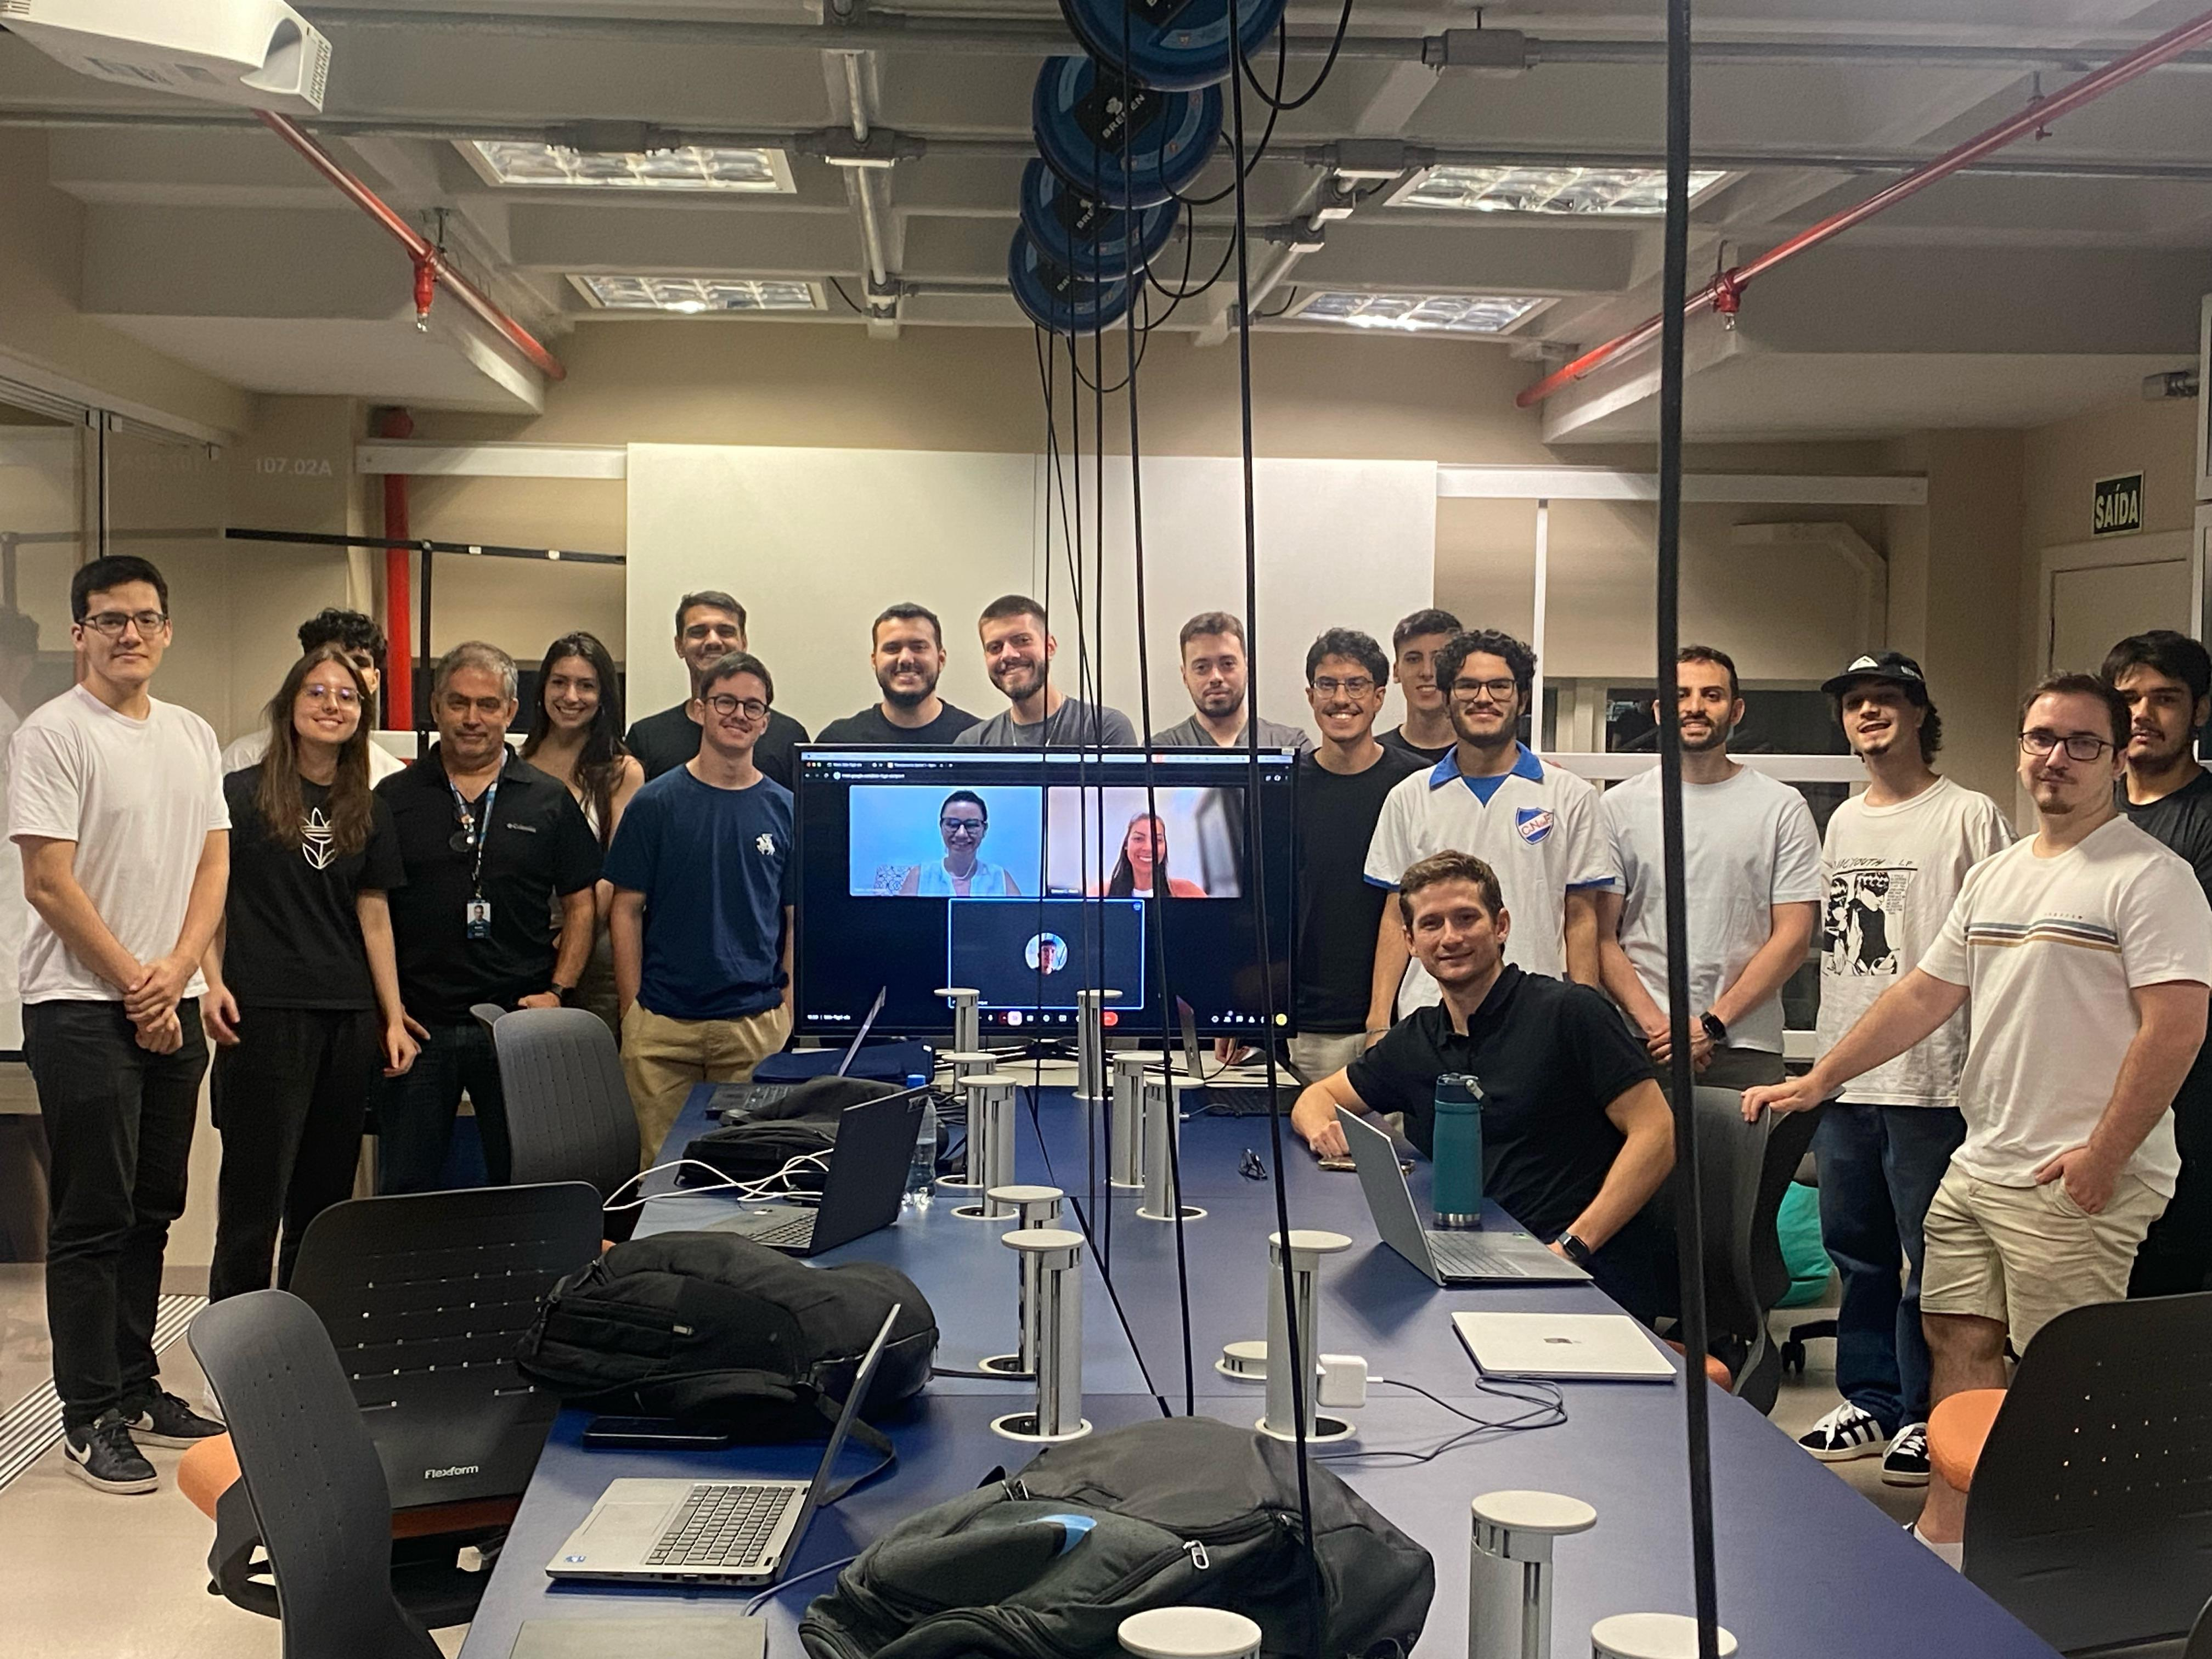
\includegraphics[width=1\linewidth]{conteudo//4 - ages III//conteudo//figures//foto-time.jpg}
    Fonte: https://tools.ages.pucrs.br/treinamentoAutoguiado/wiki/-/tree/main
\end{figure}
\section[Desenvolvimento do Projeto]{Desenvolvimento do Projeto}

\subsection{Repositório do Código Fonte do Projeto}
  Para este projeto foram utilizados dois repositórios separados, ambos foram mantidos no GitLab das AGES. A separação deles foi feita em frontend, que foi programado na linguagem Typescript\cite{typescript} utilizando a ferramenta React\cite{react} e TailwindCSS\cite{tailwindcss} e backend, sendo programado em Java\cite{java}, utilizando a ferramenta Springboot\cite{springboot}.

    \begin{itemize}
      \item Programa Manejo de Estresse frontend: https://tools.ages.pucrs.br/idoso-mais/idoso-mais-frontend
      \item Programa Manejo de Estresse backend: https://tools.ages.pucrs.br/idoso-mais/idoso-mais-backend
    \end{itemize}

\subsection{Banco de Dados Utilizado}
  Durante a Sprint 0 foram elencadas algumas das possíveis tecnologias que poderíamos utilizar durante essa AGES, porém, como todos os integrantes possuíam algum conhecimento e familiaridade com bancos de dados relacionais, acabamos por escolher o PostgreSQL\cite{postgresql}, que é uma ferramenta amplamente conhecida, de fácil uso e configuração.
  
  Como esse projeto possui um frontend mais estático, nosso banco de dados serviria muito mais para armazenar nossos usuários e em qual etapa de progressão eles pararam de utilizar a plataforma, permitindo que fosse feito um rastreio de progresso. Isso seria feito a partir da tabela "user\_progress", que iria possuir todas as entradas dos "modules\_items" que já foram completos pelo usuário. Além disso, a plataforma também possui questões a serem respondidas acerca do que foi aprendido durante a etapa, as respostas dessas perguntas seriam armazenadas na tabela "answers", permitindo que essas respostas fossem expostas ao usuário em um momento posterior.

    \begin{itemize}
      \item https://tools.ages.pucrs.br/treinamentoAutoguiado/wiki/-/wikis/database
    \end{itemize}

    \begin{figure}[H]
        \centering
        \small
        \caption{Esquema Banco de Dados Programa Manejo de Estresse}
        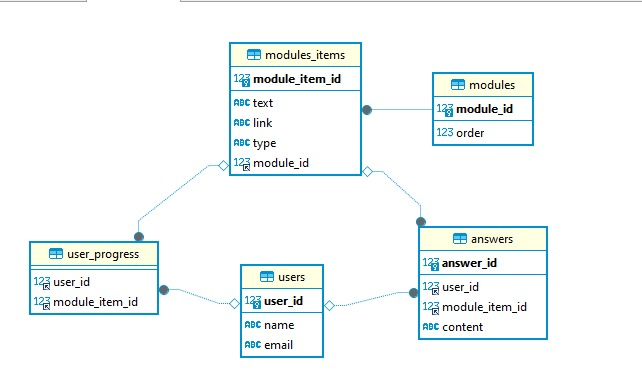
\includegraphics[width=1\linewidth]{conteudo//4 - ages III//conteudo//figures//bd.jpg}
        Fonte: https://tools.ages.pucrs.br/treinamentoAutoguiado/wiki/-/wikis/database
    \end{figure}

\subsection{Arquitetura Utilizada}
  Para disponibilizar a ferramenta, nós utilizamos a AWS\cite{aws}, que é um serviço cloud de fácil uso. Para fazer a instanciação dos recursos a serem utilizados foi usada a ferramenta Terraform, que permite fazer a definição de Infrastructure as Code, permitindo ver a arquitetura de forma mais clara e bem definida.

Inicialmente haviamos planejado uma arquitetura mais robusta, utilizando diversos serviços, porém, limitações foram impostas pela \ac{ages} e tivemos que simplificar o projeto, logo, acabamos utilizando uma EC2 para fazer o hosting tanto do backend e banco de dados, quanto do frontend e, também, para executar nossas pipelines com o GitLab Runner.

Por consequencia dessa escolha, a aplicação ficou com uma capacidade de usuários menor, dado que estava tendo que dividir poder computacional e espaço de armazenamento entre diversas aplicações. Além disso, não conseguimos criar um endereço customizado para a máquina, sendo necessário utilizar o endereço de IP público pré definido.

    \begin{itemize}
      \item https://tools.ages.pucrs.br/treinamentoAutoguiado/wiki/-/wikis/arquitetura
    \end{itemize}

    \begin{figure}[H]
        \centering
        \small
        \caption{Esquema de Recursos AWS Programa Manejos de Estresse}
        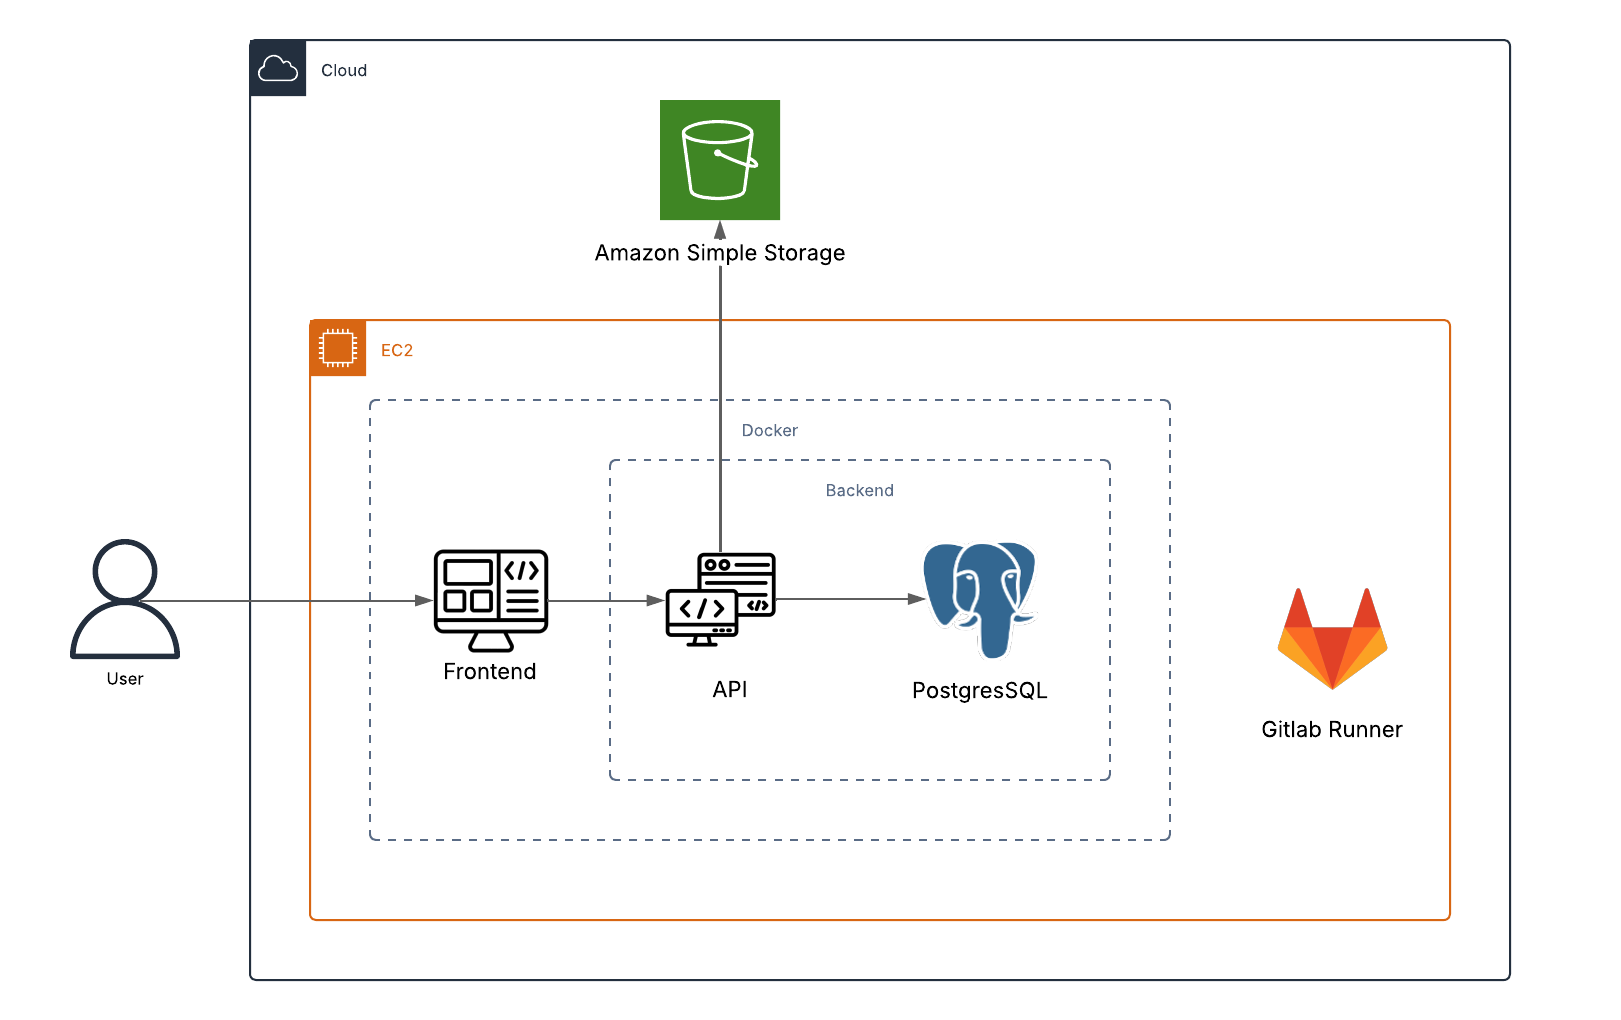
\includegraphics[width=1\linewidth]{conteudo//4 - ages III//conteudo//figures//arquitetura-aws.png}
        Fonte: https://tools.ages.pucrs.br/treinamentoAutoguiado/wiki/-/wikis/arquitetura
    \end{figure}

\subsection{Protótipos das Telas Desenvolvidas}
  Diferentemente das minhas duas primeiras AGES, nesse time, não possíamos um integrante que tivesse grande afinidade com Figma e um conhecimento amplo de design, somando isso ao fato de que precisavamos desenvolver uma plataforma web responsiva, tarefas desafiadoras foram apresentadas à equipe acerca do design, porém, acabamos conseguindo atingir um resultado que nos deixou bastante satisfeitos, fazendo utilização do design pattern utilizado na empresa das stakeholders e tentando seguir padrões de estilização mais amigáveis dada a natureza e o objetivo da plataforma.

    \begin{itemize}
      \item https://tools.ages.pucrs.br/treinamentoAutoguiado/wiki/-/tree/main TODO
    \end{itemize}

\subsection{Tecnologias Utilizadas}
  Para o desenvolvimento do projeto, foram utilizadas duas linguagens com diferentes técnologias para cada uma. Para o frontend foi utilizado o Typescript com a ferramenta React para o desenvolvimento e o Tailwind CSS para a estilização. Para o Backend optamos por utilizar a linguagem Java com o framework Sprintboot por serem amplamente conhecidas e de fácil uso, apesar da necessidade de fazer uma grande quantidade de boilerplate. Para o banco de dados foi escolhido o PostgreSQL por ser uma ferramenta de banco de dados relacional e de fácil uso, além de ser conhecida por diversos membros da equipe. Além das técnologias citadas, também foi utilizado o Docker para facilitar o desenvolvimento da aplicação, no qual executamos tanto o nosso banco de dados quanto nossa API dentro de um container, permitindo a fácil inicialização do projeto e que o mesmo fosse sempre executado sob as mesmas condições de configuração.

    \begin{itemize}
      \item https://tools.ages.pucrs.br/treinamentoAutoguiado/wiki/-/wikis/arquitetura
    \end{itemize}

\section[Atividades Desempenhadas Pelo Aluno no Projeto]{Atividades Desempenhadas Pelo Aluno no Projeto}

\subsection{Sprint 0}

Na Sprint 0 foi feito o primeiro contato com uma das nossas stakeholders, conhecemos da origem da plataforma, como a ideia surgiu e como ela funciona. Também ficamos sabendo de que a plataforma já possuia uma estrutura definida e que isso não poderia ser alterado, dado que se tratava de um processo definido e criado por uma psicóloga. Também ficamos sabendo que existia um documento com diversas definições de design e recebemos a informação que seria necessário criar uma plataforma com o menor custo possível, dado que seria algo a ser disponibilizado para a sociadade de forma gratuita.

A partir disso começamos a projetar o design da plataforma no figma, porém, diferentemente das minhas experiências passadas na AGES, dessa vez não possuíamos um integrante com uma grande afinidade com o Figma e conhecimento de design, o que dificultou consideravelmente as atividades previstas para a Sprint 0. Por esse motivo, resolvemos iniciar trabalhando individualmente e criar diversos designs diferentes para que no próximo encontro fosse possível definir quais nós mais gostamos e seguir em diante.

Conseguimos facilmente chegar uma definição de design para a plataforma no formato mobile, porém estavamos com bastante dificuldade para o desktop, porém com o empenho de alguns integrantes conseguimos chegar a um resultado satisfatório para mostrar às stakeholders, mas algumas alterações ainda seriam necessárias e isso foi passado para a Sprint 1 como um débito.

Além do design, utilizamos a Sprint 0 para fazer a definição de quais técnologias seriam utilizadas no projeto a partir de votação em quais técnologias eram mais conhecidas e quais despertavam o interesse dos integrantes da equipe. Ao final da votação acabamos ficando com Typescript com React e Tailwind CSS para o frontend e Java com Springboot para o backend, assim como PostgreSQL para o banco de dados.

Após definir as técnologias, nós, AGES III começamos a projetar a base do projeto, inicializando o código e definindo dependências, além de fornecer exemplos para que os AGES I e II pudessem seguir quando fossem realizar suas tasks.
\subsection{Sprint 1}

No início da Sprint 1 tivemos que decidir entre trabalhar em squads ou apenas delegar tasks e quem necessitasse de ajuda com sua task iria atrás dos AGES III e IV para pedir auxilio. Acabamos indo com a segunda opção por causa da grande quantidade de AGES III na nossa equipe, o que iria dificultar a separação de squads.

Enquanto delegávamos as tasks notamos que nosso projeto era relativamente simples programaticamente e que não seria necessário atribuir tasks aos AGES III, permitindo que nós agissimos como "coringas" que poderiam ajudar em qualquer momento e também iríamos supervisionar tasks mais complicadas, além de fazer todos os reviews e correções necessárias no código.

Com relação às regras de envio de código, definimos que dois reviews seriam necessários para aprovar as mudanças. Um review de um AGES III com especialidade na área e um outro review dos AGES IV para termos certeza que nada passou despercebido. Isso funcionou muito bem, dado que não tivemos nenhum código com problemas enviado para nossa branch principal.

Durante o andamento eu fiquei incubido com o objetivo de modelar nossa estrutura cloud dado que a pessoa com maior conhecimento nessa área e experiência com AWS. Para isso defini uma estrutura que facilitasse ao máximo os nossos deploys, evitando que ocorressem problemas de última hora e que o máximo de etapas pudessem ser automatizadas. Assim montei um sistema que utilizaria o AWS Amplify para fazer o hosting do nosso frontend, permitindo um fácil build e deploy do nosso projeto, porém, não notei que o recurso não tinha suporte direto para ambientes self-hosted, o que dificultaria um pouco o processo de automação de deploy. Para o backend optei por utilizar uma EC2 que iria executar tanto nosso banco de dados quanto a nossa API. Essa EC2 estaria conectada a um API Gateway que iria ser a porta de entrada para nossa API, redirecionando todas chamadas para a máquina virtual. Para fazer o instanciamento de todos esses recursos na AWS criei uma configuração utilizando Terraform e enviei para o Arquiteto de Software da AGES para que pudesse ser aprovado.

Durante a Sprint 1 ocorreram pedidos de mudança nas especificações, o que significou que, infelizmente, alguns trabalhar que já haviam sido feitos deveriam ser alterados, porém, apesar de ser um acontecimento chato, não apresentou um grande problema dado que ainda estávamos no inicio do projeto. Também tivemos alguns problemas de comunicação entre alguns membros da equipe, o que resultou em algumas complicações na divisão de tasks, porém tudo ocorreu bem e conseguimos entregar mais tasks do que foram planejadas para a Sprint 1, se concluindo com stakeholders felizes e satisfeitas.
\subsection{Sprint 2}

No início da Sprint 2 foi debatido se iríamos continuar a trabalhar sem squads e apenas delegando tasks e resolvemos continuar com o sistema de delegar tasks, monitorar o progresso dos colegas e, caso alguém tivesse dúvidas ou precisasse de ajuda com o desenvolvimento poderia pedir ajuda no Discord ou WhatsApp. Essa decisão foi feita por termos tido um ótimo resultado na Sprint 1 e optamos por não atrapalhar a dinâmica que estava se formando entre os integrantes da equipe.

Enquanto era feita a divisão de tasks, foi alertado que essa seria a Sprint mais díficil e que caso as tasks dela não fossem bem implementadas o resto do projeto iria ser muito mais complicado do que o esperado, o que adicionou um certo peso e seriedade sobre o trabalho que seriad desenvolvido. Isso se dava ao fato da nossa aplicação ser relativamente modular, o que implicava na necessidade de uma ferramenta que fizesse uma boa organização do que era recebido da nossa \ac{api} e, também, em uma boa organização na forma de guardar os dados que seriam expostos no frontend, isso exigiria um trabalho com constante comunicação entre os desenvolvedores do backend e do frontend.

Durante essa Sprint dei procedimento à criação dos nossos recursos na AWS. Apesar de ter feito o envio com o Terraform completo do que seria usado, ocorreram problemas com a instanciação dos recursos utilizando a ferramenta e acabei pedindo para o arquiteto da AGES criar os recursos manualmente para mim. Quando recebi os acessos, a primeira coisa que fiz foi inicializar nosso backend na máquina EC2 utilizando Docker e realizar os testes necessários. Após isso tentei fazer o setup do Gitlab Runner também utilizando Docker, porém, após seguir diversos tutoriais que encontrei, nenhum funcionou. Por isso decidi fazer a instalação direto na máquina e tomei todas precauções possíveis para minimizar o entrelaçamento dos ambientes. Quando estava terminando de criar o Runner do frontend o Gitlab da AGES ficou fora do ar, o que impossibilitou a progressão por mais 3 dias.

Ao fim da Sprint consegui finalizar o que era necessário e coloquei a aplicação no ar, o que facilitou muito a apresentação para as clientes, dado que as mesmas não poderiam comparecer presencialmente na reunião. Com isso, pudemos receber um feedback detalhado do que precisaria ser corrigido e o que estava bom. Apesar da instabilidade no Gitlab conseguimos realizar uma entrega satisfatória para as clientes que se mostraram extremamente felizes com a velocidade e qualidade com a qual a aplicação estava sendo desenvolvida.
\subsection{Sprint 3}
Com o início dessa Sprint foram, novamente, divididas as tasks que cada integrante da equipe seria responsável por desenvolver. Aproveitei para avisar o time de que grande parte dessa Sprint eu estaria ausente por conta de uma viagem proveniente de uma competição que eu e alguns amigos ganhamos com a \ac{uci} e, por isso, estaria nos Estados Unidos durante a próxima semana o que poderia dificultar no desenvolvimento da minha task.

Durante essa Sprint eu, juntamente com os outros \ac{ages} III, recebemos as tasks de mapear e organizar o items dos módulos a partir do documento apresentado pelas stakeholders. Eu imaginei que não conseguiria finalizar minha task até o dia da viagem, por isso, acabei conversando com um outro \ac{ages} III para que ele pudesse ver alguém para assumir a parte da minha task que faltava.

Além dessa task, eu recebi um outro trabalho para fazer, criar um \ac{s3} e adicionar nele os áudios que deveriam ser apresentados no frontend. Acabei preferindo focar em finalizar essa task, já que eu era o único com experiência em \ac{aws} no time. Assim, enviei uma requisição para o arquiteto da \ac{ages} pedindo que o mesmo criasse um \ac{s3} para que pudessemos utilizar. Enquanto aguardava fui tentando mapear quais áudios deveriam ir para o \ac{s3} e em qual ordem seriam utilizados, para que pudesse manter o armazenamento de forma organizada e que permitisse acessos eficientes. Quando recebi acesso ao \ac{s3} apenas precisei fazer o upload dos arquivos e definir os meta-dados.

No fim acabei precisando repassar minha task de mapear os items dos módulos para outro colega, dado que minha viagem iria percorrer até o sábado anterior à entrega.

Quando retornei de viagem, já sabia que seria necessário fazer o deploy das alterações para a \ac{aws}, porém não esperava encontrar um problema com o espaço de armazenamento da máquina enquanto fazia isso. Eu, juntamente com outro \ac{ages} III ficamos por algumas horas tentando resolver o problema até descobrirmos que isso estava ocorrendo por conta do docker, que não estava fazendo a remoção dos caches de building, mantendo todos os arquivos que utilizávamos para montar qualquer container duplicado dentro da máquina. Apesar dos problemas conseguimos fazer o deploy do front e backend.

Ao fim da Sprint 3 fizemos, no geral, um bom trabalho, não tivemos débitos técnicos, porém, diversos erros foram encontrados, o que resultaria em uma quantidade de trabalho bem maior que o esperado para a próxima e última Sprint. Apesar dos erros, as stakeholders pareceram bem felizes com a entrega.
\subsection{Sprint 4}

No início da Sprint 4 foram, novamente, separadas as tasks para cada integrante da equipe, porém não teríamos quase nada de novas features, essa Sprint seria composta em sua maior parte por correção de bugs.

Durante essa Sprint eu fiquei responsável por corrigir alguns bugs que tínhamos encontrado com os audios e as imagens e por fazer uma integração com a \ac{api} Lumiar, uma \ac{api} da empresa das stakeholders. Essa \ac{api} deveria receber algumas informações dos usuários em alguns casos pré-determinados.

Como já haviamos recebido um documento listando todas as coisas que estavam erradas no projeto, resolvi começar arrumando os audios e imagens. Foi bem simples fazer as correções necessárias, dado que era basicamente mudar a nomenclatura no \ac{s3} e atualizar nosso seed do banco de dados.

A parte difícil dessa Sprint foi quando tive de fazer a integração. Inicialmente fiz uma chamada para a \ac{api} Lumiar toda vez que um usuário finalizava um módulo, porém, mais para o fim da Sprint recebemos um documento informando que essa integração deveria ser feita algumas vezes horas após o último acesso do usuário, mais especificamente 24 horas e 72 horas depois. Essa \ac{api} iria enviar uma notificação por WhatsApp para o usuário incentivando-o a voltar e terminar o módulo.

Como nunca havia feito isso, precisei pesquisar e pensar um pouco e cheguei a conclusão que usar cron expressions seria uma boa alterantiva. Pedi ajuda ao professor orientador perguntando se ele sabia de alguma tecnologia que pudesse ser usada de forma fácil e ele me reportou que o próprio Springboot possui essa utilidade. Com essas informações montei uma lógica que executava uma vez por dia e verificava quais usuários deveria ser enviados para a \ac{api} Lumiar.

Após a entrega as stakeholders se mostraram muito felizes com o resultado final do projeto, porém encontraram alguns erros no fluxo do guia montado por elas. Assim, pedimos, novamente, um reporte de todas alterações que seriam necessárias.

Notamos que diversas coisas que foram reportadas como erradas, foram, na verdade, alteradas durante a Sprint 4 para ficarem como pedido no documento enviando anteriormente, mas, refizemos algumas alterações para ficarem do gosto das stakeholders.
\section[Conclusão]{Conclusão}

Em suma, com a junção das experiências obtidas como \ac{ages} I, II e III, posso afirmar que cada time tem uma dinâmica com relação à divisão de squads e organização de tasks. Diferentemente das minhas duas experiências anteriores, nessa \ac{ages} não foram feitas squads, mas sim divisão de tasks diretamente para cada integrante da equipe. Acredito fortemente que essa organização não deve ser comumente usada e depende fortemente da proatividade dos colegas do time.

Com relação à minha atuação como \ac{ages} III, posso concluir que, apesar de termos muitos \ac{ages} III, consegui aplicar meu conhecimento técnico de forma positiva para o projeto, auxiliando os colegas que precisavam e assumindo o controle quando necessário. Apesar de não ter tido muito contato com o frontend da aplicação sabia constantemente o que estava sendo desenvolvido tanto no front quanto no backend e estava observando e avaliando o que poderia dar errado.

No quesito social, ou seja, softskill, eu acredito ter crescido muito desde minha \ac{ages} II, pois consegui ter um melhor contato com os colegas e repassar de uma maneira mais didática o meu conhecimento técnico, mostrando uma clara evolução dessa habilidade.
  %\chapter[AGES IV --- “NOME DO PROJETO XXXX”]{AGES IV --- “NOME DO PROJETO XXXX”}

Para cada projeto o aluno deverá argumentar sobre o que foi desenvolvido,
seu aprendizado com críticas e autocrítica.

\section[Introdução]{Introdução}

  Na introdução o aluno deve apresentar os seguintes itens: Descrição do Projeto,
Stakeholders do Projeto, Período de Execução, Professor Orientador e uma foto do
time.
\section[Desenvolvimento do Projeto]{Desenvolvimento do Projeto}

\subsection{Repositório do Código Fonte do Projeto}
  Deverão ser apresentados os links da Wiki, com uma breve descrição.

\subsection{Banco de Dados Utilizado}
  Deverão ser apresentados os links da Wiki, com uma breve descrição.

\subsection{Arquitetura Utilizada}
  Deverão ser apresentados os links da Wiki, com uma breve descrição.

\subsection{Protótipos das Telas Desenvolvidas}
  Deverão ser apresentados os links da Wiki, com uma breve descrição.

\subsection{Tecnologias Utilizadas}
  Deverão ser apresentados os links da Wiki, com uma breve descrição.
  
  As tecnologias citadas deverão ter referências bibliográficas.

\section[Atividades Desempenhadas Pelo Aluno no Projeto]{Atividades Desempenhadas Pelo Aluno no Projeto}

\subsection{Sprint 0}

No mínimo uma página contendo tudo que o aluno fez na Sprint 0.
\subsection{Sprint 1}

No mínimo uma página contendo tudo que o aluno fez na Sprint 1.
\subsection{Sprint 2}

No mínimo uma página contendo tudo que o aluno fez na Sprint 2.
\subsection{Sprint 3}
No mínimo uma página contendo tudo que o aluno fez na Sprint 3.
\subsection{Sprint 4}

No mínimo uma página contendo tudo que o aluno fez na Sprint 4.
\section[Conclusão]{Conclusão}

Neste item o aluno deverá refletir sobre:
\begin{itemize}
    \item Crítica e autocrítica em relação a sua atuação no projeto na parte técnica como na parte de soft skills.
    \item Comente o relacionamento entre as disciplinas cursadas e a AGES.
    \item Este projeto foi o melhor projeto trabalhado? Justifique.
    \item Relate as lições aprendidas (retrospectiva pessoal):
    \begin{itemize}
        \item O que foi positivo no projeto.
        \item O que podia ter sido melhor (em ternos de banco, desenvolvimento, arquitetura, soft skills....)
    \end{itemize}
\end{itemize}
(No mínimo uma página de relato)
  %\chapter[Considerações Finais]{CONSIDERAÇÕES FINAIS}

As considerações finais referem-se a trajetória do aluno no curso, onde se
expõe o fechamento da narrativa e são apresentados os resultados alcançados.

Este item é somente para os AGES IV.\

Em particular, espera-se neste capítulo:
\begin{itemize}
  \item{contribuições que o curso trouxe para a sua evolução profissional} 
  \begin{itemize}
    \item competências (o que) e habilidades desenvolvidas (como),
    (hardskills e softskills);
    \item lições aprendidas (o que deu certo, o que deu errado);
  \end{itemize}
  
  \item uma reflexão sobre a visão do aluno sobre a prática da Engenharia de
Software, como era no início de sua trajetória, e que visão ele tem hoje;
  
  \item eventuais comentários que deseje adicionar;
  
  \item sugestão de melhorias, críticas e elogios em relação a AGES.\
\end{itemize}

(No mínimo uma página de relato)

  % Configuração de referência bibliográfica:
\printbibliography[title=Referências]


  %\chapter*{Apêndices}

\textbf{APÊNDICE A} – Exemplo1: Análise dos relatórios mensais de uso do serviço de
renovação de empréstimos.
\end{document}